% \documentclass[handout,table]{beamer}
\documentclass[table,dvipsnames,aspectratio=169]{beamer}
\usepackage[utf8]{inputenc}
\usepackage[spanish]{babel}
\usepackage{beamerthemeshadow}
\usepackage{times}
\usepackage{graphicx}
\usepackage{amsmath,amssymb,amsfonts,latexsym,stmaryrd}
\usepackage{tabularx}
\usepackage{xcolor}
\usepackage{color, colortbl}
\usepackage{tikz}
\usepackage{shadow} 
\usepackage{listings}
\usepackage{../res/mips}
\usepackage{../res/lstlangarm}
\usepackage{multirow}
\usepackage{rotating}
\usepackage{ragged2e} % para justificar texto
\usepackage{fancybox}
\usepackage{shadow}
\usepackage{multicol}
\usepackage[binary-units]{siunitx}
\usepackage[absolute,overlay]{textpos}
\usepackage[most]{tcolorbox}
\usepackage{cancel}
  \setlength{\TPHorizModule}{1mm}
  \setlength{\TPVertModule}{1mm}
\usetikzlibrary{calc}
\pgfdeclarelayer{background}
\pgfdeclarelayer{foreground}
\pgfsetlayers{background,main,foreground}

\setbeamertemplate{navigation symbols}{}

%%%%%%%%%%%%%%%%%%%%%%%%%%%%%%%%%%%%%%%%%%%%%%%%%%%%%%%%%%%%%%%%%%%%%%%%%%%%%%%%%%%%%%%%
%Para hacer cajas de texto con sombras lindas
\definecolor{ShadowColor}{RGB}{130,150,190}


\makeatletter
\newcommand\Cshadowbox{\VerbBox\@Cshadowbox}
\def\@Cshadowbox#1{%
  \setbox\@fancybox\hbox{\fbox{#1}}%
  \leavevmode\vbox{%
    \offinterlineskip
    \dimen@=\shadowsize
    \advance\dimen@ .5\fboxrule
    \hbox{\copy\@fancybox\kern.5\fboxrule\lower\shadowsize\hbox{%
      \color{ShadowColor}\vrule \@height\ht\@fancybox \@depth\dp\@fancybox \@width\dimen@}}%
    \vskip\dimexpr-\dimen@+0.5\fboxrule\relax
    \moveright\shadowsize\vbox{%
      \color{ShadowColor}\hrule \@width\wd\@fancybox \@height\dimen@}}}
\makeatother
%%%%%%%%%%%%%%%%%%%%%%%%%%%%%%%%%%%%%%%%%%%%%%%%%%%%%%%%%%%%%%%%%%%%%%%%%%%%%%%%%%%%%%%%%%%%


\graphicspath{
{../img/}
}

\newenvironment{changemargin}[2]{%
\begin{list}{}{%
\setlength{\topsep}{0pt}%
\setlength{\leftmargin}{#1}%
\setlength{\rightmargin}{#2}%
\setlength{\listparindent}{\parindent}%
\setlength{\itemindent}{\parindent}%
\setlength{\parsep}{\parskip}%
}%
\item[]}{\end{list}}


\mode<presentation>{
	\usetheme{Copenhagen}
	\useoutertheme{infolines}

}
\setbeamercovered{invisible}

\parskip=1ex

\title[Introducción Arquitectura y Organización]{Introducción a la Arquitectura y Organización de Computadores}

\author{Alejandro Furfaro}
\date{\today}

\begin{document}

\lstset{
	frame=Ltb,
	framerule=10pt,
	aboveskip=0.5cm,
	framextopmargin=0pt,
	framexbottommargin=0pt,
	framexleftmargin=0.8cm,
	framesep=0pt,
	rulesep=.4pt,
	backgroundcolor=,%\color{gray97},
	rulesepcolor=\color{black},
	language=[ARM]Assembler,
	captionpos=b,
	tabsize=6,
	frame=lines,
	keywordstyle=\color{blue},
	commentstyle=\color{purple},
	stringstyle=\color{red},
	numbers=none,%left,
	numberstyle=\tiny,
	numbersep=5pt,
	breaklines=true,
	showstringspaces=false,
	basicstyle=\small,
	emph={label},
	framerule=0pt,
}

\vspace{0.5cm}
\begin{figure}[h]
  \centering 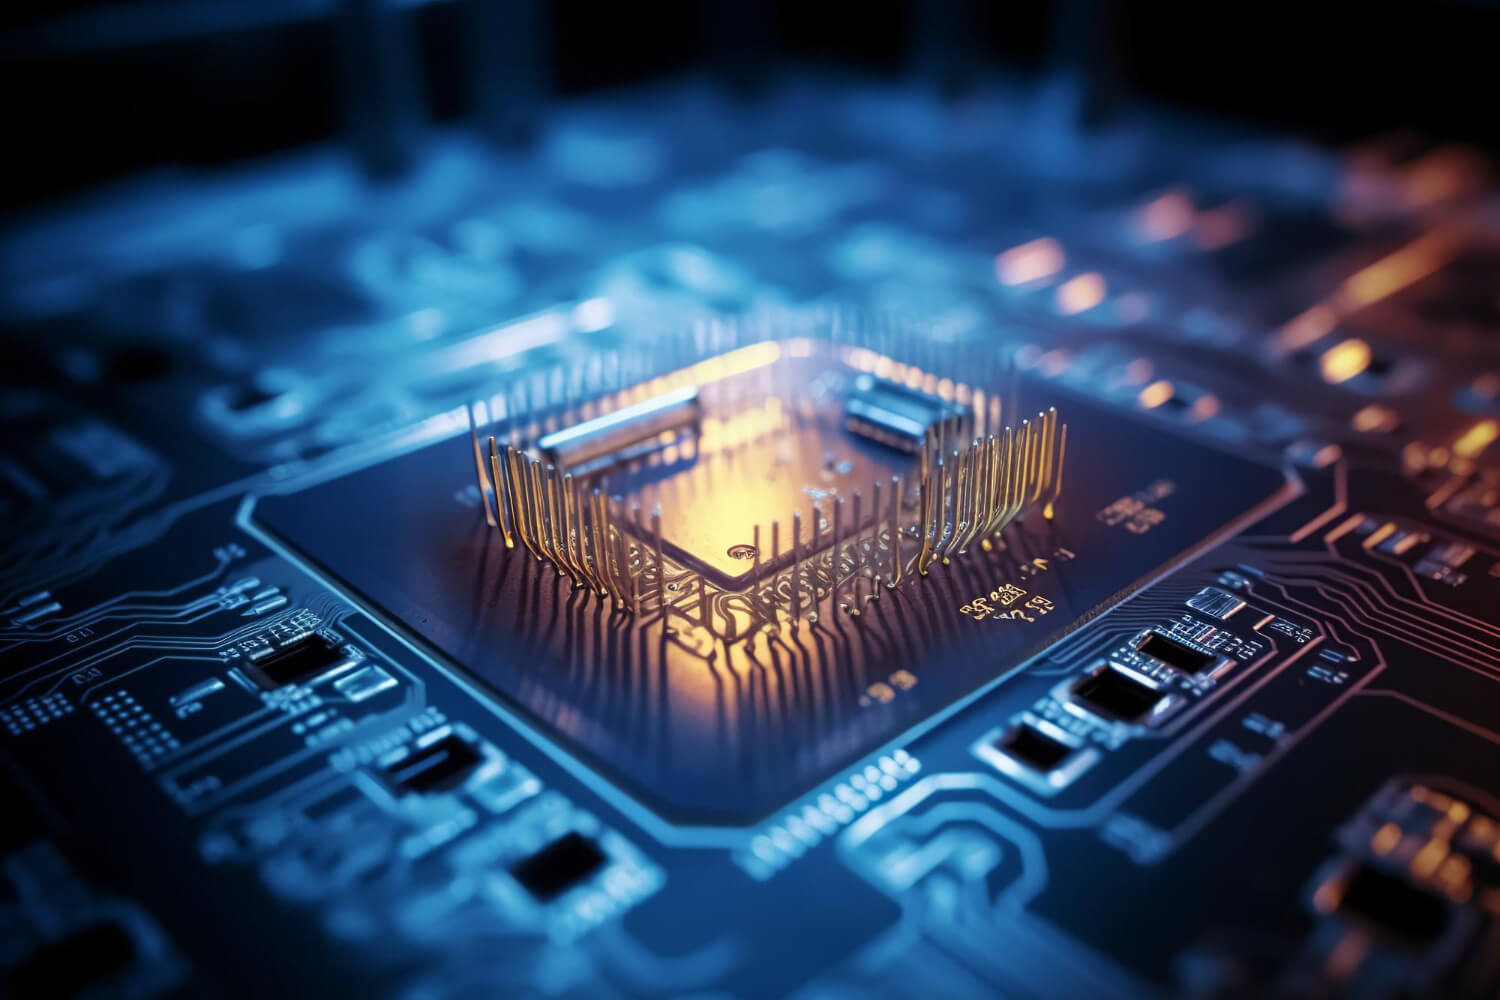
\includegraphics [width =0.4\textwidth]{VLSI.jpg}
  % \includegraphics [width = 2.5cm]{Barcelona.jpg}
\end{figure}
\vspace{-2cm}
\titlepage
  
\begin{frame}{Contenido}
 \vspace{-0.5cm}
 \begin{multicols}{2}
  \setcounter{tocdepth}{2} 
  \footnotesize \tableofcontents
 \end{multicols}
\end{frame} 

\definecolor{OliveGreen}{RGB}{2,80,1}
\definecolor{LigthOrange}{RGB}{255,255,200}
\definecolor{gray97}{gray}{.97}
\definecolor{Gray}{RGB}{171,174,178}
\definecolor{orange}{RGB}{255,127,0}

\definecolor{furfiBlue}{rgb}{0.35, 0.31, 0.81}
\definecolor{furfiGreen}{rgb}{0.0, 0.66, 0.42}
\definecolor{furfiGray}{rgb}{0.66, 0.66, 0.66}

%Comandos para tipografías especiales a nombres relevantes

\AtBeginSubsection[]
{
  \begin{frame}
    \setcounter{tocdepth}{2}  
    \footnotesize \tableofcontents[currentsection, sectionstyle=show/shaded, subsectionstyle=show/shaded/hide]
  \end{frame}
}

\section{Pioneros}
\subsection{Introducción histórica para empezar a entender algunos ``\textit{porque}''}
\begin{frame}{¿Quien diseñó el primer computador de propósito general?}
 \begin{textblock*}{\textwidth}(0.4cm,1.15cm)
  \begin{itemize}[<+->] \justifying \setlength{\parskip}{6mm}
   \item ¿Fue Alan Turing durante los años 30?
   \item ¿Fue Von Newmann en los años 40?
   \item ¿Fueron los alemanes durante la 2da. Guerra Mundial?
   \item .... Frío ....
  \end{itemize}
 \end{textblock*}
\end{frame}

\begin{frame}{Fue en el sigo XIX.... }
 \begin{textblock*}{.95\textwidth}(0.4cm,1.15cm)
  \centering 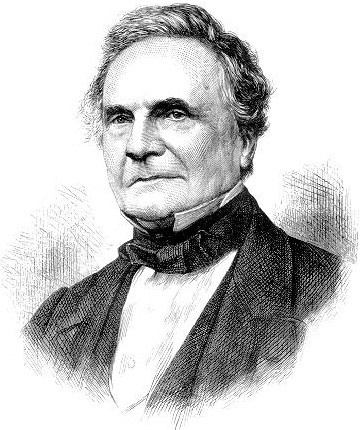
\includegraphics[width=0.4\textwidth]{babage1.jpg}\\
  \textbf{Charles Babbage 26/12/1791 - 18/10/1871}
 \end{textblock*}
\end{frame}

\begin{frame}{Máquina Analítica (1837)}
 \begin{textblock*}{.95\textwidth}(0.4cm,1.15cm)
 \centering 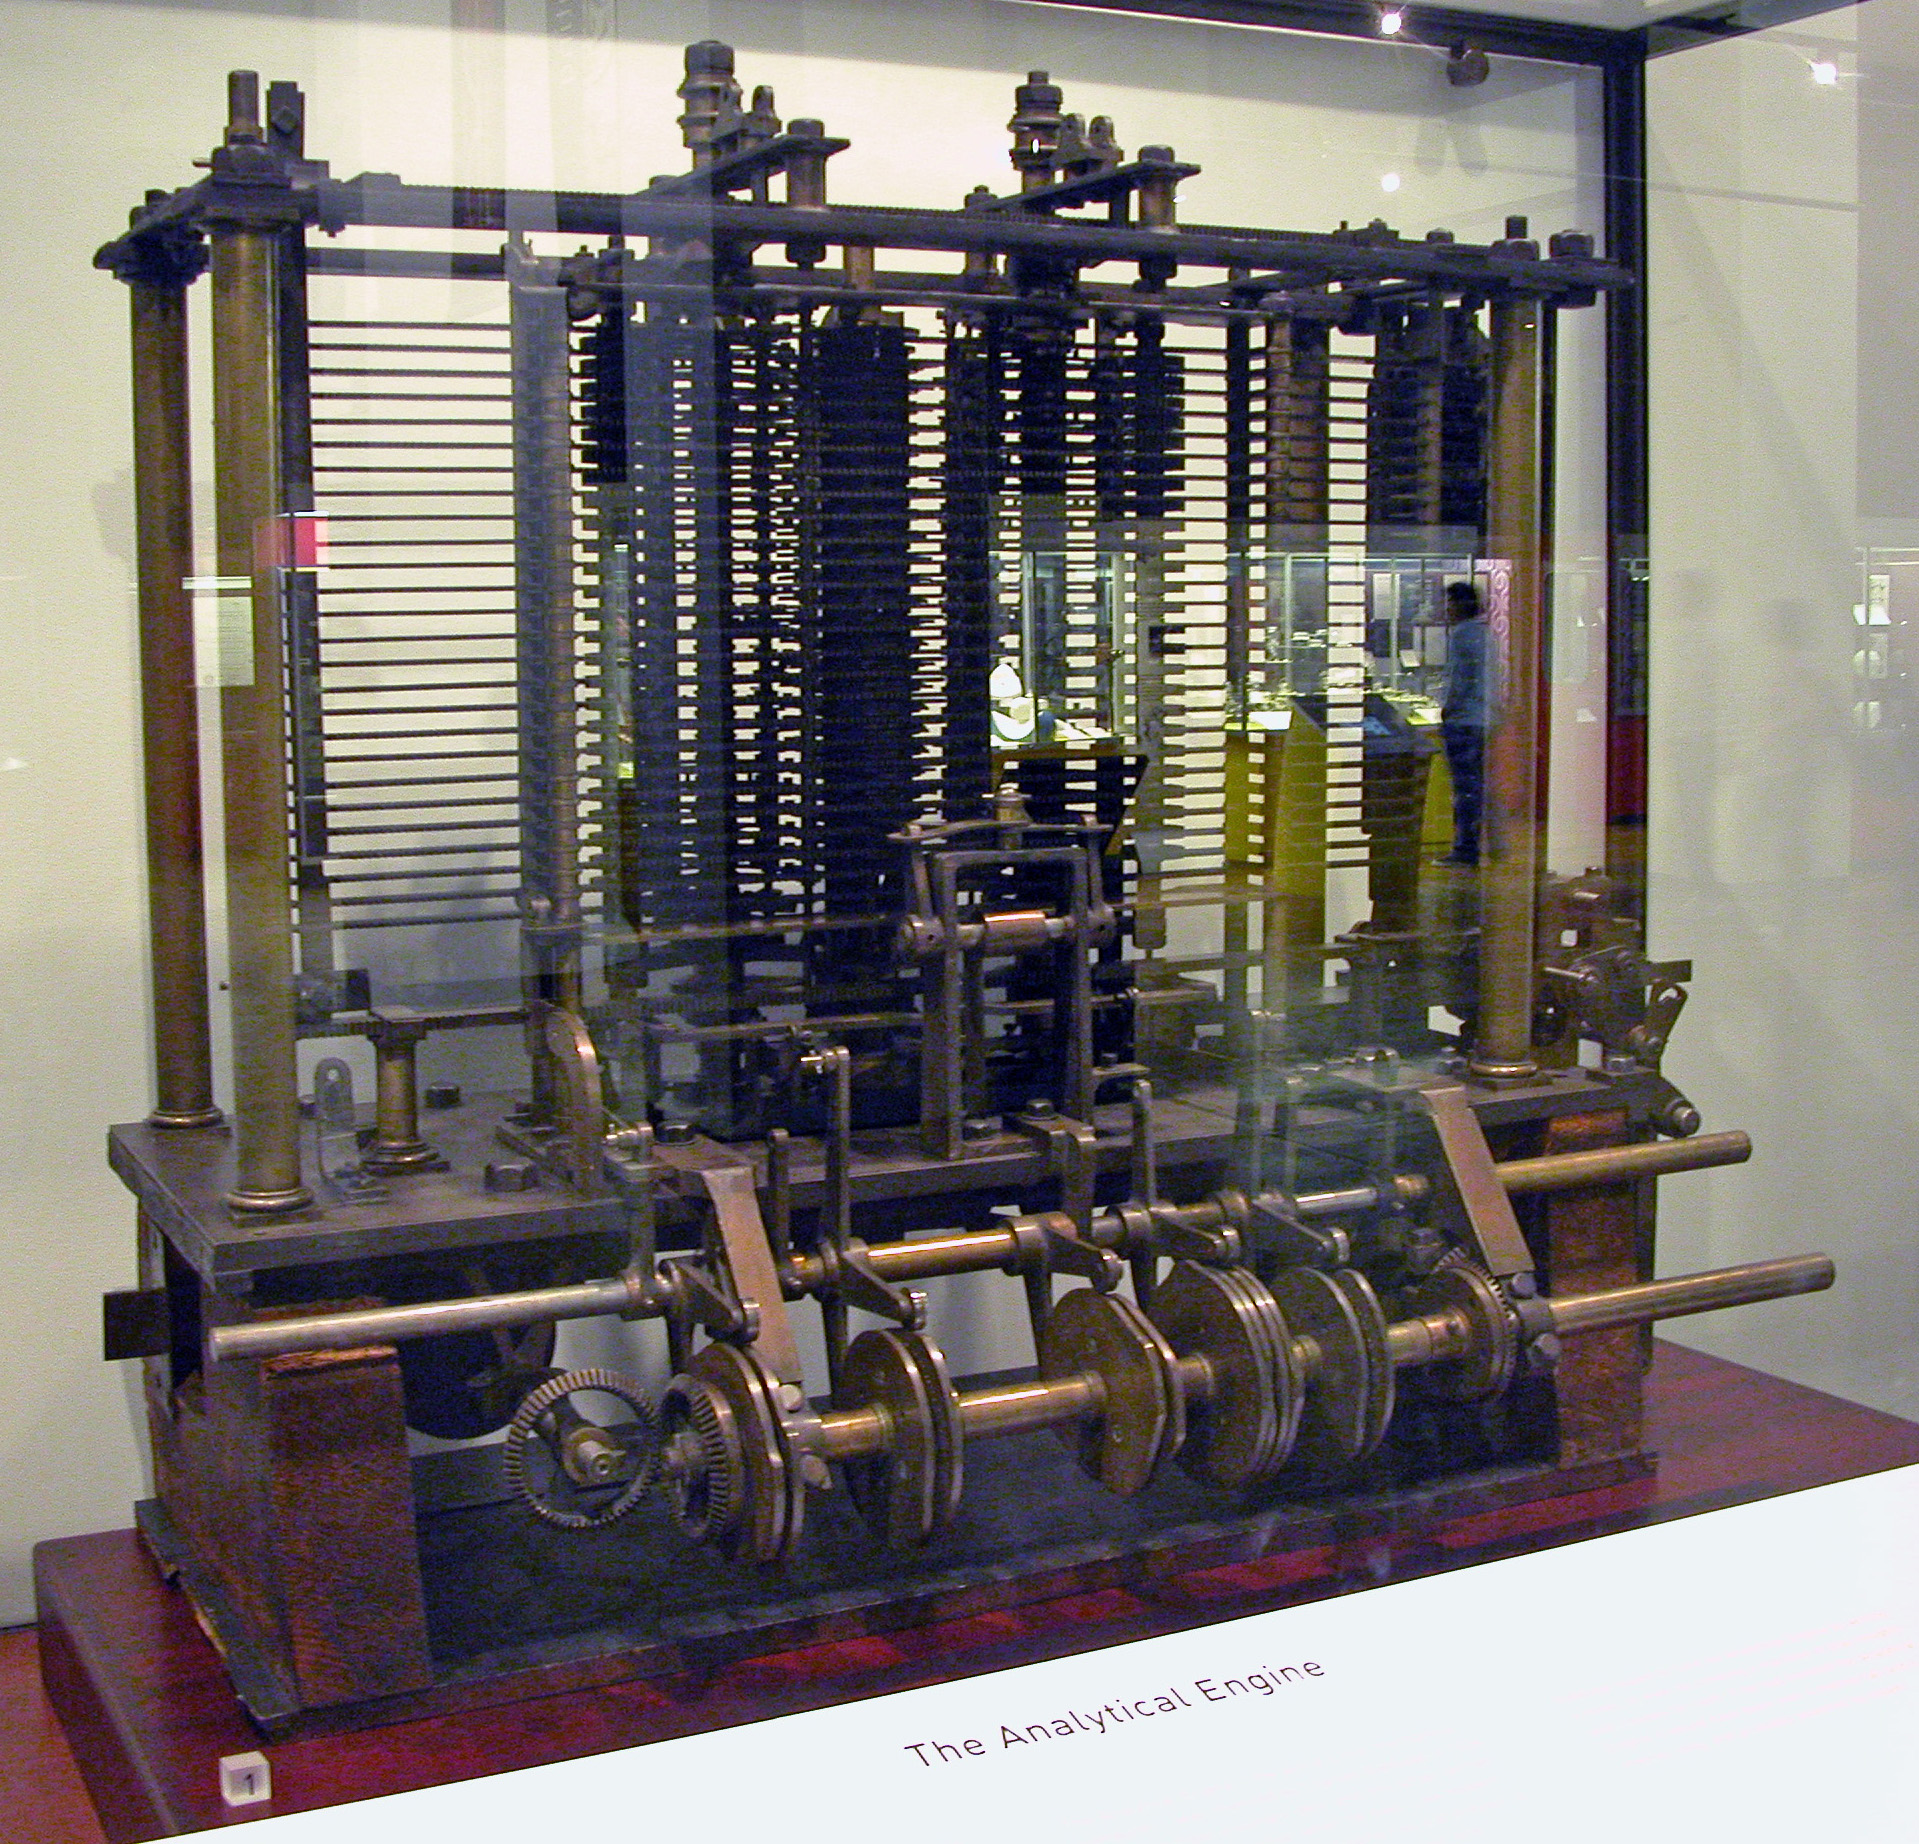
\includegraphics[width=0.4\textwidth]{AnalyticalMachine_Babbage_London.jpg}\\
 Analitical Machine. \scriptsize Foto: \textcopyright De Bruno Barral (ByB), CC BY-SA 2.5, \url{https://commons.wikimedia.org/w/index.php?curid=6839854}
 \end{textblock*}
\end{frame}

\begin{frame}{Diferential Engine (14 de Junio de 1821)}
 \begin{textblock*}{.95\textwidth}(0.4cm,1.15cm)
  \centering 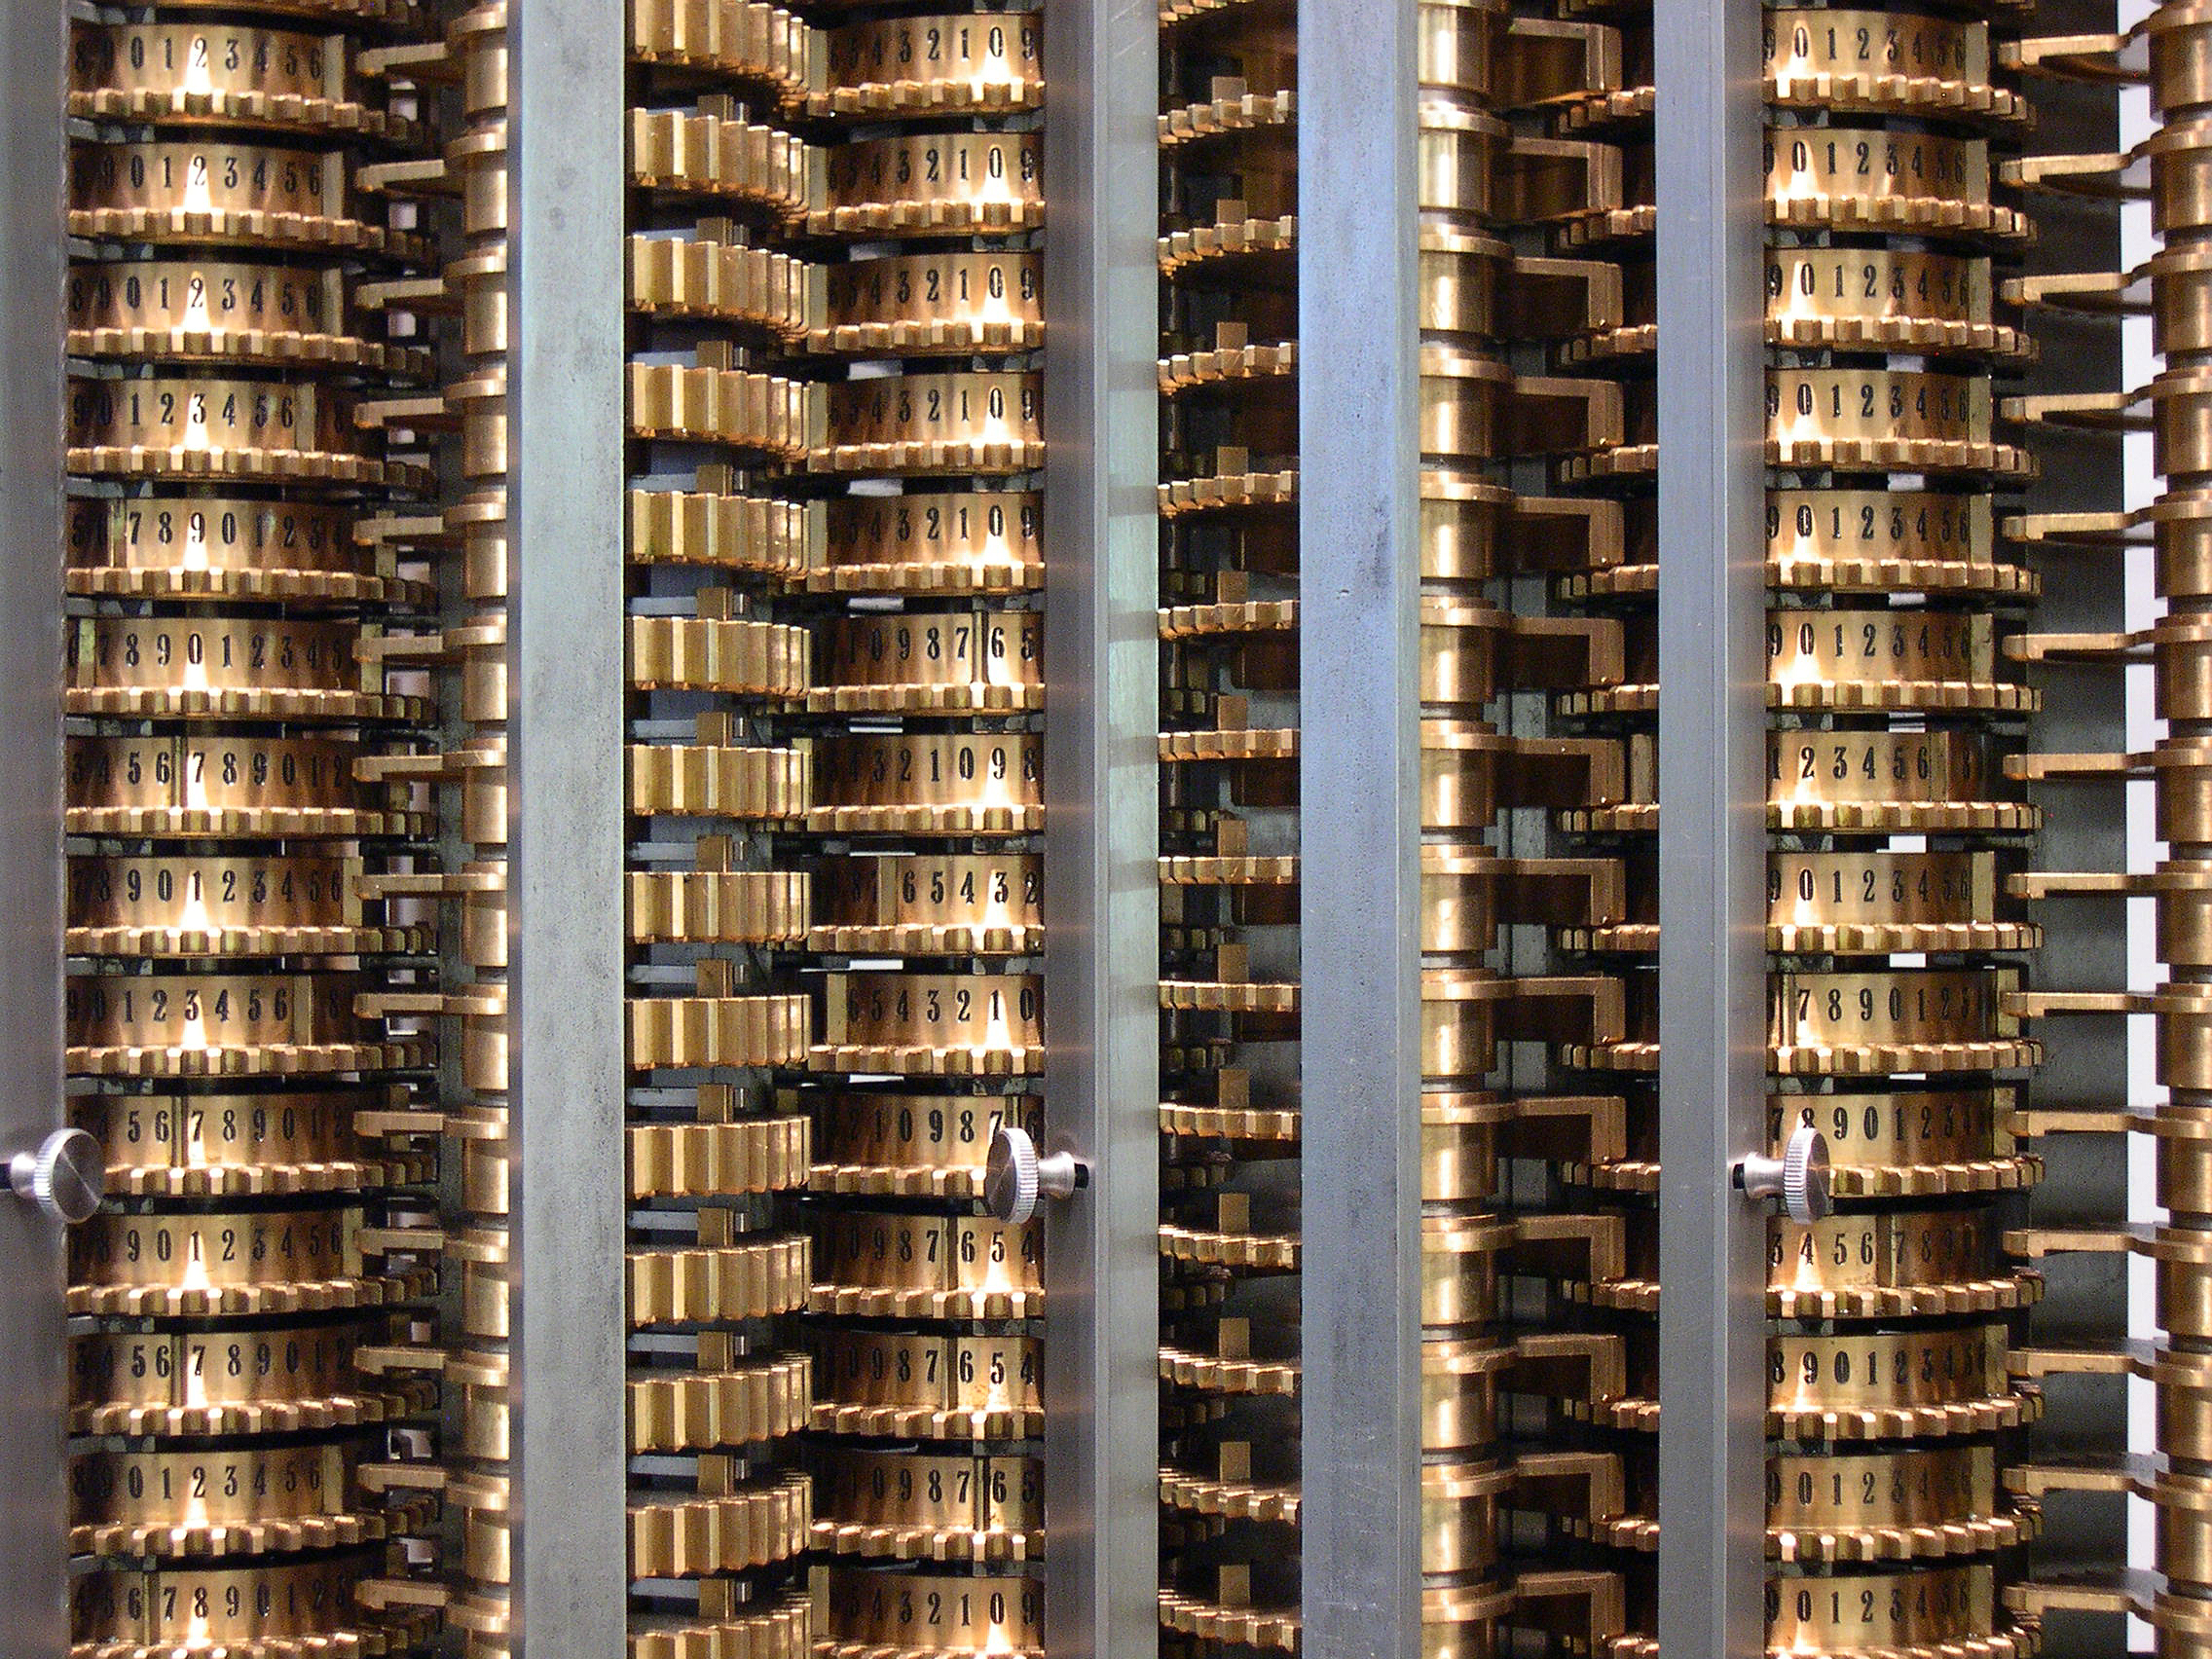
\includegraphics[width=0.55\textwidth]{LondonScienceMuseumsReplicaDifferenceEngine.jpg}\\
  Diferential Engine. \scriptsize Foto: \textcopyright De Carsten Ullrich - Trabajo propio, CC BY-SA 2.5, \url{https://commons.wikimedia.org/w/index.php?curid=851017}
 \end{textblock*}
\end{frame}

\begin{frame}{Z3: (1941) Primer Computador Programable}
 \begin{textblock*}{.95\textwidth}(0.4cm,1.3cm)
  \centering 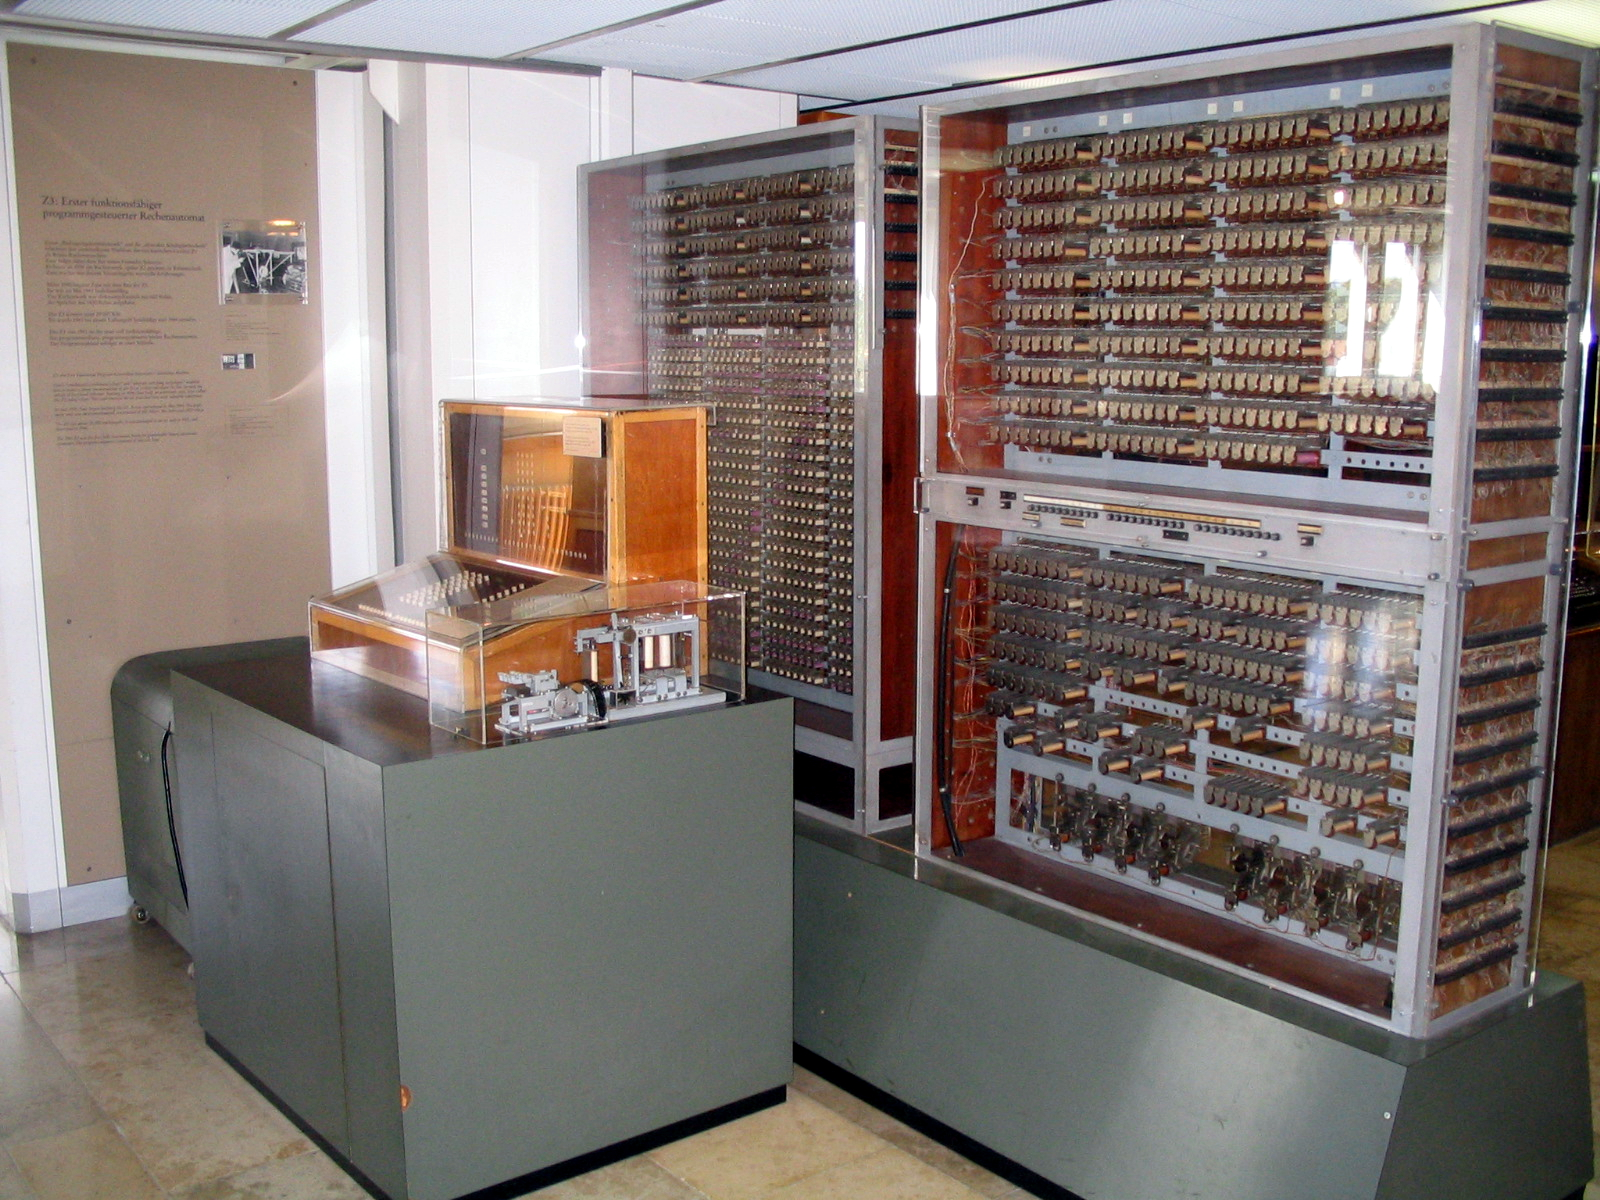
\includegraphics[width=0.55\textwidth]{Z3_Deutsches_Museum.JPG}\\
  Réplica del Computador Z3. \scriptsize Foto: \textcopyright De Venusianer, CC BY-SA 3.0, \url{https://commons.wikimedia.org/w/index.php?curid=3632073}
 \end{textblock*}
\end{frame}

\begin{frame}{La Máquina de Turing}
 \begin{textblock*}{.45\textwidth}(0.4cm,1.3cm)
  \centering 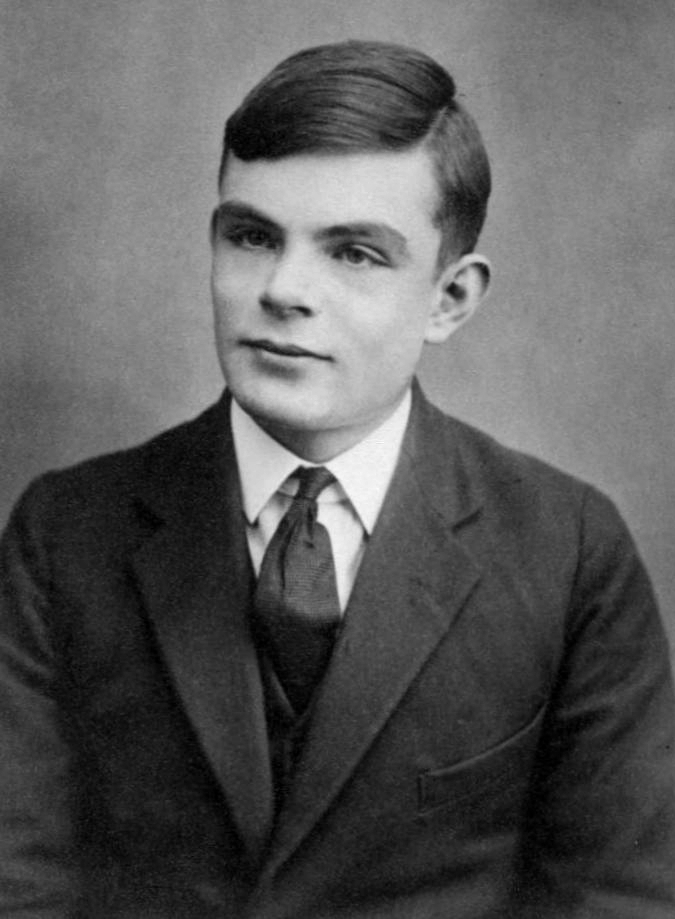
\includegraphics[width=0.54\textwidth]{Alan_Turing_Aged_16.jpg}\\
  Alan Turing. \scriptsize Foto: \textcopyright De Desconocido - \url{http://www.turingarchive.org/viewer/?id=521\&title=4}, Dominio público, \url{https://commons.wikimedia.org/w/index.php?curid=22828488}
 \end{textblock*}
 \begin{textblock*}{.6\textwidth}(6.4cm , 1.15cm)
 \begin{itemize} \parskip 0.4cm
  \item Hasta que Alan Turing enunció en 1936 su\\
  modelo teórico conocido como Máquina de\\
  Turing, \textcolor{furfiBlue}{no se disponía de un marco formal}\\
  para trabajar en ciencias de la computación.
  \item La Máquina de Turing es un \textcolor{furfiBlue}{modelo matemático}\\
  implementable mediante un autómata, que tiene\\
  la capacidad de implementar cualquier problema\\
  matemático, que pueda ser expresado a través\\
  de un \textcolor{furfiBlue}{algoritmo}.
  \end{itemize}
 \end{textblock*}
\end{frame}

\begin{frame}{Componentes La Máquina de Turing}
 \begin{textblock*}{\textwidth}(0.4cm,1.15cm)
  \begin{itemize}[<+->] \justifying
   \item Una \textcolor{furfiBlue}{cinta} de longitud infinita dividida en celdas contiguas.
   \item Un \textcolor{furfiBlue}{cabezal} que puede avanzar o retroceder la cinta en un paso discreto.\\
   (un paso = una celda), y que además puede leer o escribir en la cinta.
   \item Un \textcolor{furfiBlue}{registro de estado}, que describe el estado en que se encuentra la máquina.\\
   {\textcolor{Gray}{\small (Turing lo asimilaba al estado mental de una persona cuando realiza un cálculo mental)}}
   \item Una \textcolor{furfiBlue}{tabla de instrucciones}, que permite en función del valor leído y eventualmente de alguna acción ingresada por el usuario:\\
   \hspace{1cm} escribir un resultado,\\
   \hspace{1cm} avanzar la cinta,\\
   \hspace{1cm} retroceder la cinta,\\
   \hspace{1cm} dejar la cinta en su mismo lugar,\\
   \hspace{1cm} y actualizar el nuevo estado en el registro de estados.
  \end{itemize}
 \end{textblock*}
\end{frame}

\begin{frame}{La Contribución fundamental de Alan Turing}
  \begin{itemize}[<+->] \setlength{\itemsep}{6mm}
   \item De éste modo, Turing proporcionó la descripción matemática de un \textcolor{furfiBlue}{dispositivo}\\
   muy simple con capacidades de \textcolor{furfiBlue}{cómputo arbitrarias}, capaz de probar capacidades\\
   de computabilidad tanto generales como particulares.
   \item La \textcolor{furfiBlue}{\textit{Completitud Turing}} de un sistema de instrucciones es la medida de su\\
   capacidad de simular una máquina de Turing.
   \item En la actualidad los lenguajes de computación utilizados son \textcolor{furfiBlue}{Turing Completos}\\
   siempre que no se considere que ejecutan sus programas en memoria finita.
  \end{itemize}
\end{frame}

\section{Evolución}
\subsection{Vorágine evolutiva}
\begin{frame}{En solo algo menos de 80 años}
 \begin{textblock*}{\textwidth}(0.4cm,1.15cm)
  \centering  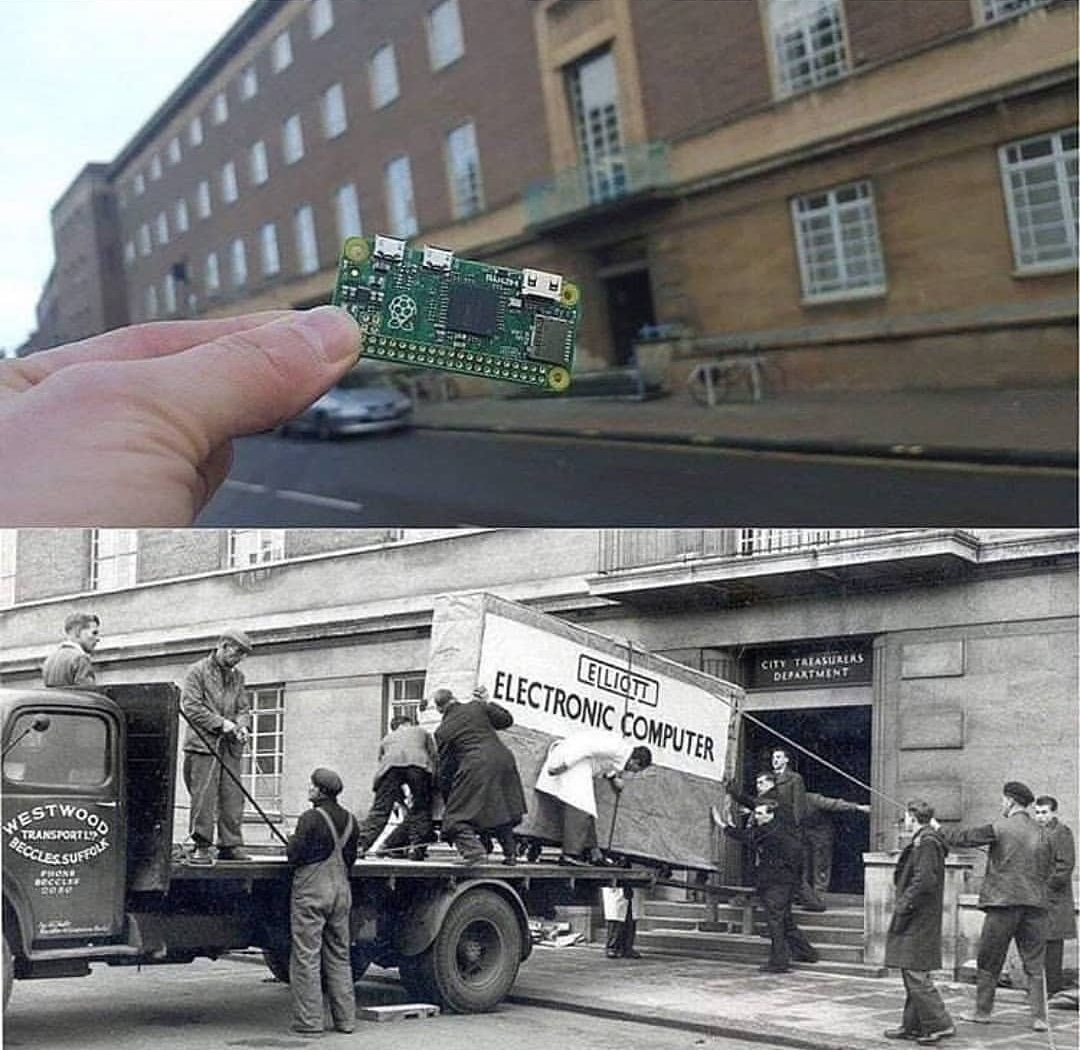
\includegraphics[width=0.5\textwidth]{Evol.jpg}
 \end{textblock*}
\end{frame}

\begin{frame}{ENIAC \textquotedblleft primer\textquotedblright Computadora de Propósito general}
 \begin{textblock*}{0.7\textwidth}(0.4cm,1.3cm)
  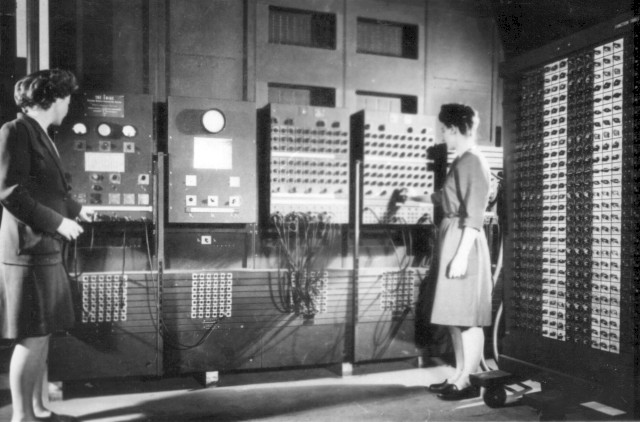
\includegraphics[width=\textwidth]{ENIAC.jpg}
 \end{textblock*}
 \only<2>{
 \begin{textblock*}{0.28\textwidth}(11.2cm,1.3cm)
 \small
  \justifying Tal parece que la Z1 desarrollada en Alemania durante la WWII fue algo anterior.\\
  \vspace{0.2cm}
  Pero fue destruida al final de la guerra por los militares alemanes.\\
  \vspace{0.2cm}
  \textcolor{furfiBlue}{ENIAC está considerada la primera}. No utilizaba programa almacenado, sino que se programaba mediante 6000 interruptores.\\
  \vspace{0.4cm}
  Consumo 160 KW.\\
  Peso: 27 Toneladas.\\
  Superficie: 167 $m^{2}$.
 \end{textblock*}
 }
\end{frame}

\begin{frame}{ENIAC BackPlane. Observar las vávulas termoiónicas}
 \begin{textblock*}{\textwidth}(0.4cm,1.2cm)
  \centering  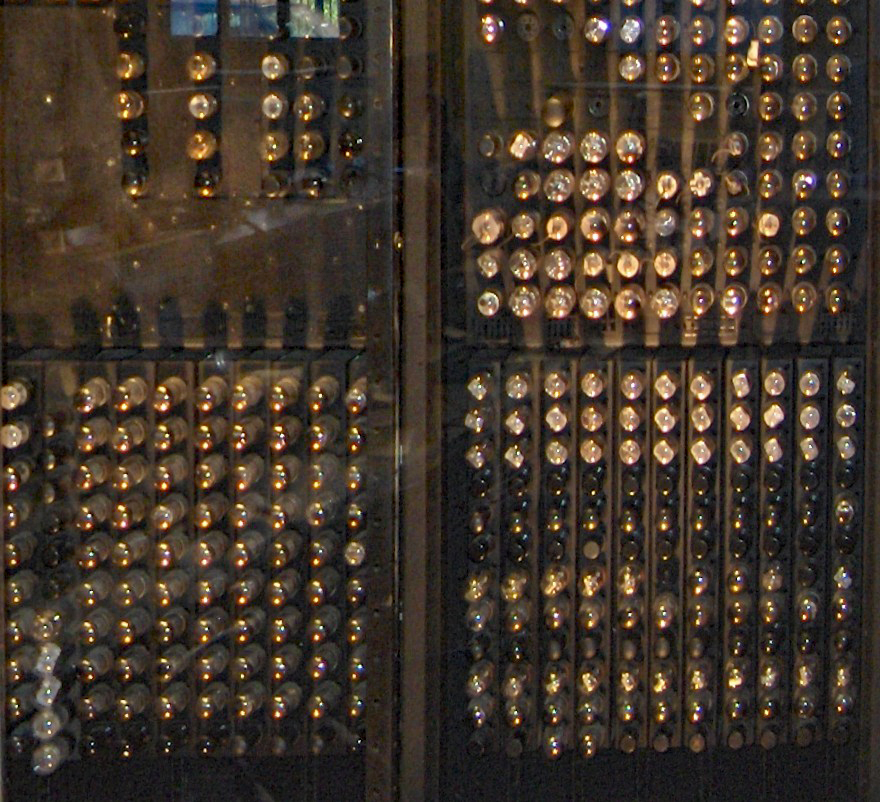
\includegraphics[width=0.53\textwidth]{ENIAC_Penn2.jpg}
 \end{textblock*}
\end{frame}

\begin{frame}{Modelo de Von Mewmann}
  \begin{itemize}[<+->] \justifying \setlength{\itemsep}{6mm}
   \item En 1945 se publica ``First Draft of a Report on the EDVAC. John Von Newmann''.
   \item Este reporte borrador describe \textcolor{furfiBlue}{la organización y arquitectura} de una máquina de cómputo binaria y electrónica en la que se detallan las características y recursos de arquitectura de los componentes principales.
   \item Tal vez su mérito principal sea el de haber sido la primer publicación de la arquitectura y organización de un computador basado en los postulados de Turing de una década antes.\\
   Obviamente la \textbf{EDVAC} (por \textbf{E}lectronic \textbf{D}iscrete \textbf{V}ariable \textbf{A}utomatic \textbf{C}omputer) era una máquina Turing completa.
  \end{itemize}
\end{frame}

\begin{frame}[t]{Modelo de Von Mewmann}
  \begin{itemize}[<+->] \justifying  \setlength{\itemsep}{6mm}
   \item Inaugurando el lema ``publish or perish'', esta arquitectura por ser la primera bien documentada, \textcolor{furfiBlue}{se convirtió en sinónimo de programa almacenado} {\small (recordemos que la máquina de Turing había postulado las bases teóricas de este concepto 9 años antes).}
   \item De modo que sin perjuicio de los valiosos aportes de Von Newmann, estos conceptos salieron de otra mente brillante: \textcolor{furfiBlue}{la de Alan Turing}.
   \item No obstante, los avances relativos de la EDVAC debidos a los trabajos de Von Newmann, y su publicación en el trabajo antes mencionado fue fundamental para la difusión del modelo de programa almacenado.
   \item Esta publicación fue muy influyente durante décadas en el diseño y concepción de computadores, y éste es su significativo aporte.
  \end{itemize}
\end{frame}

\begin{frame}{Modelo de Von Mewmann}
\vspace{0.2cm}
\centering 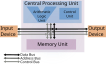
\includegraphics[width=0.65\textwidth]{VonNewmann.pdf}\\
\small Modelo simplificado de Von Newmann: Tres unidades unidas por tres buses.
\end{frame}

\begin{frame}{Modelo de Von Mewmann}
  \small
  Esta organización fue dominante durante la primer y segunda generación de Computadores.\\
  Sus principales componentes se describen a continuación:
  \begin{description}[<+(1)->][\textbf{\textit{Central Arithmetic (CA)}}:] \justifying \parskip 0.4cm
   \item [\textbf{\textit{Central Arithmetic (CA)}}:] Una Unidad de Procesamiento Aritmético Lógica y Registros.
   \item [\textbf{\textit{Central Control (CC)}}:] Implementación de la máquina de estados, con registro de\\
                                                   instrucciones y registro  Contador de Programa.
   \item [\textbf{\textit{Memory (M)}}:] Almacena el código y los Datos. Dos cuestiones:\\
   (1) Esta idea ya estaba en la \textbf{ENIAC} y en otros diseños anteriores, y\\
   (2) Con el tiempo se advirtió que este escenario limita la performance ya que no permite leer una instrucción y un dato a la vez, escenario conocido como ``Von Newmann bottleneck''.
  \end{description}
\end{frame}

\begin{frame}{Modelo de Von Mewmann}
  \begin{description}[<+->][\textit{\textbf{Memoria Externa (R)}}:]\justifying \parskip 0.4cm
   \item [\textbf{\textit{Entrada (I)}}:] Se trata de mecanismos para que se puedan ingresar al\\
                                          computador comandos y datos desde el exterior.
   \item [\textbf{\textit{Salida (O)}}:] Se trata de mecanismos para que el computador pueda\\
                                         enviar resultados hacia el mundo exterior.
   \item [\textit{\textbf{Memoria Externa (R)}}:] Se trata de un medio de almacenamiento de mayor capacidad\\
                                                  que la Unidad de Memoria {\small (en donde solo están el código y los datos del programa en ejecución)}.\\
                                                  En la Memoria externa podemos tener una colección de programas y datos para copiar de a una vez en la Unidad de Memoria y lanzar a ejecutar. Es lo que hoy conocemos como Storage. Por entonces se trataba de Cintas perforadas por ejemplo.
  \end{description}
\end{frame}


\begin{frame}{Modelo de Von Meumann}
  \begin{enumerate}[<+->]\justifying \setlength{\itemsep}{6mm}
  \item Modelo de programa almacenado.
  \item Datos y programa en el mismo (único) banco de memoria.
  \item Máquina de estados perpétua:\\
  \vspace{0.2cm}
  \begin{center}
  \uncover<3->{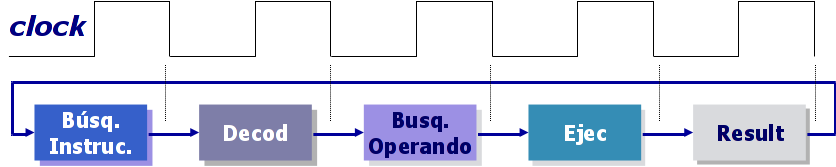
\includegraphics[width=0.75\textwidth]{cicloInstruc.pdf}}
  \end{center}
  \item No está claro cual fue la primera implementación, pero Manchester Baby, IBM-SSEC, EDVAC, BINAC, entre otras fueron de las primeras (alrededor de 1948 todas ellas)
 \end{enumerate}
\end{frame}

\begin{frame}{Modelo Harvard }
 \begin{textblock*}{\textwidth}(0.4cm,1.2cm)
  \begin{itemize}[<+(1)->]\justifying \parskip 0.4cm
   \item Cuando Von Newmann publicó el reporte de la EDVAC, tal vez era difícil imaginar que en solo cuestión de algo mas de dos décadas, se necesitaría leer desde la memoria un código de operación y los datos necesarios para llevarla adelante \textbf{al mismo tiempo} (o al menos que todo se comporte como si así fuese).
   \item \textcolor{furfiBlue}{El postulado de Von Newmann ``una única Unidad de Memoria para datos y código'', definitivamente no encaja en este nuevo paradigma.}
   \item En este nuevo escenario, una memoria que almacene ambas entidades se transforma inevitablemente en un \textcolor{furfiBlue}{cuello de botella}.
   \item Y de este modo se rebautiza al modelo de la EDVAC como ``Von Newmann bottleneck''. ¿Injusto?, tal vez, pero asi se lo conoce desde entonces
  \end{itemize}
 \end{textblock*}
\end{frame}

\begin{frame}{Modelo Harvard}
 \begin{textblock*}{\textwidth}(0.4cm,1.2cm)
  \begin{itemize}[<+->]\justifying\parskip 0.2cm
   \item Recién por entonces y ante ese problema concreto, algunos diseñadores repararon en el diseño de la \textbf{Mark I}, un computador electromecánico desarrollado por IBM y la Universidad de Harvard entre 1939 y 1944. 
   \item \textcolor{furfiBlue}{Ni siquiera un computador de la primer generación, y obviamente anterior a la \textbf{EDVAC}.}
   \item ¿Que podía tener de interesante esta pieza de museo compuesta de 760.000 engranajes, 800km de cables, basada en la máquina analítica de Babagge, que \textbf{trabajaba en Decimal}, y que se tomaba 0.3 a 10 segundos por cada cálculo? %(no obstante lo cual se utilizó hasta 1959...)
   \item Esta reliquia, que no era electrónica ni binaria, tenía la solución al ``Von Newmann bottleneck''. Así son las cosas\dots
   \item Su código ingresaba mediante una cinta de papel perforada, y los operandos mediante contadores electromecánicos. \textcolor{furfiBlue}{Es decir, las instrucciones y los datos ingresan por data paths diferentes.}
  \end{itemize}
 \end{textblock*}
\end{frame}

\begin{frame}{Modelo  Harvard }
\begin{block}{\textbf{\underline{Conclusiones}}}
\begin{itemize}[<+(1)->]\justifying
 \item Un computador tiene organización Harvard \textbf{\color{red}cuando las instrucciones y los datos se leen desde memorias físicamente diferentes, y por caminos de señal físicamente diferentes.}
 \item Esto permite utilizar memorias de tecnología y organización diferente para instrucciones y para datos, y mapas de direcciones individuales para cada caso, y \textbf{\color{red} caminos de señal (buses) independientes}.
 \item O sea podemos tener dos direcciones 0x00000000 de memoria: una para instrucciones y otra para datos. La memoria de instrucciones podría estar organizada en palabras de 32 bits y la de datos en palabras de 8 bits. 
 \textcolor{furfiGreen}{E igualmente todo funciona.}
\end{itemize}
\end{block}
\end{frame}

\begin{frame}{Modelo Harvard }
 \begin{textblock*}{\textwidth}(0.4cm,1.2cm)
  \centering 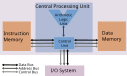
\includegraphics[width=0.6\textwidth]{Harvard.pdf}\\
\small Modelo Harvard. Mapas y buses de memoria diferentes para Instrucciones y Datos
 \end{textblock*}
\end{frame}

\begin{frame}{Modelo Harvard }
 \begin{textblock*}{\textwidth}(0.4cm,1.2cm)
  \begin{itemize}[<+->] \justifying \parskip 0.2cm
   \item \textcolor{furfiBlue}{Los microprocesadores actuales parecieran presentar al usuario una organización acorde al modelo de Von Newmann.}
   \item Sin embargo como veremos en pocas clase más, por razones de performance utilizan desde la década del 90 una tecnología denominada \textcolor{furfiBlue}{split cache}: dividir los primeros niveles de memoria cache en una de Instrucciones y otra de datos, con sendos buses independientes para accederlas en paralelo. \textcolor{furfiGreen}{Esto es Harvard}.
   \item Sin embargo, los niveles de memoria más externos almacenan instrucciones y datos juntos. \textcolor{furfiBlue}{Esto es Von Newmann}.
   \item El sub-sistema de memoria cache está diseñado y dimensionado de modo que se resuelvan en éste la mayoría de los accesos a memoria de parte de las CPUs.\\
   Un valor típico de \textcolor{furfiGreen}{eficiencia de un cache Nivel 1 es 80\%}, es decir que la mayor parte de los acceso a memoria se resuelven en una memoria organizada de acuerdo al modelo de Harvard.
   \end{itemize}
 \end{textblock*}
\end{frame}

\begin{frame}{Modelo Harvard }
 \begin{textblock*}{\textwidth}(0.4cm,1.2cm)
  \begin{itemize}[<+->] \justifying \parskip 0.2cm
   \item La única razón por la que ni siquiera el primer nivel de cache es \textcolor{furfiBlue}{``estrictamente\\
   Harvard'' se debe que el programador ``ve'' un solo espacio de direccionamiento} de\\
   memoria en lugar de ver uno para datos y otro para código. Esta división la realiza\\
   el sistema Cache en forma transparente.
   \item Los primeros modelos de microprocesadores basados en arquitectura Harvard\\
   se dieron en la década del 80 con el advenimiento de los DSP {\small (Procesadores de Señales Digitales)}, que requerían un alto nivel de paralelismo. {\small \textcolor{furfiBlue}{Estos, de momento, son los únicos procesadores puramente Harvard.}}
   \item Los procesadores de propósito general actuales, y últimamente algún que otro\\
   microcontrolador CORTEX-M, trabajan con \textcolor{furfiBlue}{split cache en el Nivel 1 de su jerarquía}\\
   de memoria, y juntan código y datos en los restantes niveles.
   \item Todos presentan al programador un mapa de direcciones de memoria único.\\
   Razón por la cual se los llama \textcolor{furfiBlue}{``casi - Von Newmann''}.
  \end{itemize}
 \end{textblock*}
\end{frame}

\subsection{La era del Silicio}
\begin{frame}{2da. Generación}
  \begin{itemize}[<+(1)->] \justifying \parskip 0.3cm
   \item Son los computadores \textcolor{furfiBlue}{transistorizados}.
   \item El transistor se implementa en 1947 en Laboratorios Bell.% (patente en Canadá en 1925) % --- DAVID: Esto no se porque es?
   \item Los primeros equipos aparecen durante fines de la década del 50.
   \item \textcolor{furfiGreen}{Ventajas: Menor consumo, menor espacio, y (a largo plazo) mejor desempeño.}
   \item Coincide con los lenguajes de Alto Nivel.\\ En 1957 se escribe el primer compilador de FORTRAN (\textbf{FOR}mula \textbf{TRAN}slator).
   \item Bell Labs presenta en 1958 la TRADIC (\textbf{TRA}nsistor, \textbf{DI}gital \textbf{C}omputer)
   \item Se consolida IBM, y nacen XEROX y DEC.
  \end{itemize}
\end{frame}

\begin{frame}{3er. Generación}
  \begin{itemize}[<+(1)->] \justifying \parskip 0.4cm
   \item Computadores basados en \textcolor{furfiBlue}{circuitos integrados (CI)}.
   \item Jack Kirby (Texas Instruments) patenta el CI junto con una implementación en 1959. (Jacobi, Siemens AG había patentado también en 1958 solo el dispositivo).
   \item En 1957 Robert Noyce funda Fairchild, y luego del patentamiento de Kirby le agrega una capa metálica que permite mejorar su conexionado.
   \item Igual que para la segunda generación, transcurriría un tiempo desde el descubrimiento del CI y la implementación de un computador de esta nueva generación.
   \item \textcolor{furfiBlue}{Los primeros equipos ven la luz en los años 60.}
   \item \textcolor{furfiGreen}{El paisaje de un salón de cómputos comienza a verse muy diferente.}
  \end{itemize}
\end{frame}

\begin{frame}{Minicomputadores de 1964.}
 \begin{textblock*}{.68\textwidth}(0.2cm,1.2cm)
  \centering 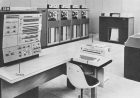
\includegraphics[width=0.63\textwidth]{IBM360.pdf}\\
  \begin{itemize}
   \item El IBM 360 cabía en una mesa.\\
   Los demás módulos son periféricos.\\
   \item Los PDP-8 de DEC también podían\\
   ubicarse sobre una mesa pequeña.
  \end{itemize}
 \end{textblock*}
 \begin{textblock*}{0.35\textwidth}(10.6cm,1.2cm)
  \centering 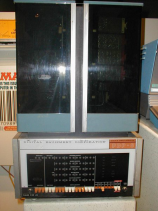
\includegraphics[width=\textwidth]{PDP-8.pdf}
 \end{textblock*}
\end{frame}

\begin{frame}{Otros problemas a resolver}
  \begin{itemize} [<+->] \justifying \parskip 2mm
   \item En los 60\texttt{'}, los usuarios de computadores demandaban disminuir el costo de\\
   actualización de sus equipos.
   \item Cada computador {\small (aun siendo del mismo fabricante)} era incompatible con los otros\\
   modelos: {\small \textcolor{furfiGray}{esto es, tenía diferentes set de instrucciones, los toolchains de desarrollo de\\
   software eran diferentes, el S.O. era diferente, la E/S era diferente, y hasta el mercado era\\
   diferente para cada modelo.}}
   \item Cada upgrade obligaba a \textcolor{furfiBlue}{reemplazar} no solo el hardware sino además el sistema operativo y las aplicaciones.
   \item Ésta dinámica dificultaba a los proveedores establecer un \textcolor{furfiBlue}{cash flow que permitiese incrementar inversiones en I+D}.
   \item La palabra \textcolor{furfiBlue}{``Compatibilidad''} comienza a escucharse en cada laboratorio de diseño de Procesadores y Computadores \textcolor{furfiGreen}{(especialmente en IBM)}.
  \end{itemize}
\end{frame}

\begin{frame}{Otros problemas a resolver}
 \begin{textblock*}{\textwidth}(0.4cm,1.05cm)
  \begin{itemize} [<+->] \justifying
   \item El diseño de un computador se divide en dos \textcolor{furfiBlue}{aspectos fundamentales}.
   \begin{enumerate}
    \item \textbf{Datapath}: Conjunto de recursos para que los números se almacenen en registros y las operaciones entre ellos se puedan ejecutar
    \item \textbf{Control}: La lógica necesaria para que las operaciones se envíen en la secuencia correcta por el \textbf{Datapath}.
   \end{enumerate}
   \item \textcolor{furfiGreen}{De los dos aspectos, el \textbf{Control} es la madre de todas las batallas.}
   \item Maurice Wilkes en IBM, tuvo una idea disruptiva para diseñar la lógica de control de un microprocesador: \textcolor{furfiBlue}{la llamó \textbf{\textit{microprogramación}} o \textbf{microcódigo}}.
   \item {\footnotesize En ese momento la memoria ROM era más barata y rápida que la RAM, así que propuso implementar el \textbf{microcódigo} en una memoria ROM, en la cual cada palabra se llama microinstrucción, y cada instrucciones se descompone en una secuencia de microinstrucciones (o pequeños programas).}
   \item En abril de 1964, IBM anuncia que todos sus modelos de mainframes IBM 360 \textcolor{furfiBlue}{se basarán en \textbf{microcódigo}}. {\footnotesize El ancho de las microinstrucciones varió desde \SI{50}{\bit} a \SI{87}{\bit}, para \textbf{Datapaths} de 8 a \SI{64}{\bit}.}
  \end{itemize}
 \end{textblock*}
\end{frame}

\begin{frame}{Microcódigo. \normalsize La solución para utilizar el mínimo de memoria}
\shabox{
\justifying
El control por \textbf{microcódigo} derivó indefectiblemente en diseño del ISA con\newline
instrucciones de \textcolor{furfiBlue}{complejidad creciente}, cargándole toda su complejidad al\newline
\textbf{microcódigo} en la CPU, y ocupando la \textcolor{furfiBlue}{menor cantidad de memoria posible}.\newline
\textcolor{furfiGray}{Con los bloques de datos no hay mucho que hacer para ahorrar memoria.\newline
Pero en el caso del código, si utilizamos menos instrucciones para un mismo\newline
algoritmo, se emplea menos cantidad de memoria.\newline}
Este \textcolor{furfiBlue}{criterio} primó en todos los diseños durante décadas. Incluso cuando\newline
Intel desarrolló la arquitectura iAPx86. Junto con el compromiso de mantener\newline
\textbf{compatibilidad}, explica porque hasta el presente \textcolor{furfiGreen}{seguimos utilizando\newline
procesadores de instrucciones complejas.}
}
\end{frame}

\begin{frame}[fragile]{Instrucciones complejas}
 \begin{textblock*}{\textwidth}(0.1cm,1.2cm)
  \begin{enumerate}[<+->] \justifying
   \item En ese contexto se han diseñado Microprocesadores capaces\\
   de integrar código de alto nivel.
   \item Ejemplos extremos: \texttt{POLY (VAX computer)}
  \end{enumerate}
  \begin{onlyenv}<3>

\lstset{
	frame=Ltb,
	framerule=0pt,
	aboveskip=0.5cm,
	framextopmargin=3pt,
	framexbottommargin=3pt,
	framexleftmargin=0.4cm,
	framesep=0pt,
	rulesep=.4pt,
	backgroundcolor=\color{gray97},
	rulesepcolor=\color{black},
	language=[95]Fortran,
	captionpos=b,
	tabsize=6,
	frame=lines,
	keywordstyle=\color{blue},
	commentstyle=\color{purple},
	stringstyle=\color{red},
	numbers=left,
	numberstyle=\tiny,
	numbersep=5pt,
	breaklines=true,
	showstringspaces=false,
	basicstyle=\small,
	emph={label},
	framerule=0pt,
}
   \begin{lstlisting}
   ! To compute P(x) = C0 + C1*x + C2*x**2
   ! where C0 = 1.0,  C1 = .5, and C2 = .25

           POLYF   X,#2,PTABLE
           .
           .
           .
   PTABLE: .FLOAT  0.25    ; C2
           .FLOAT  0.5     ; C1
           .FLOAT  1.0     ; C0
   \end{lstlisting}
  \end{onlyenv}
 \end{textblock*}
\end{frame}

\begin{frame}{La 3er. Generación produjo los Minicomputadores}
\begin{block}{Minicomputadores}
\justifying
\textcolor{furfiBlue}{Costaban un orden menos que las enormes computadores transistorizados, y\\
aumentaban en el mismo orden su potencia de cálculo.}\\
\bigskip
El descenso en el costo, permite fabricar en serie al menos algunos \textcolor{furfiBlue}{miles de equipos},\\
hecho que imprime \textcolor{furfiGreen}{impulso al desarrollo de la industria}.\\
\bigskip
Este mayor poder de cómputo del hardware posibilita el desarrollo de aplicaciones más\\
complejas, evidenciando los \textcolor{furfiBlue}{inconvenientes de los lenguajes de programación} como\\
Fortran, y la falta de metodologías de desarrollo.
\end{block}
\end{frame}

\begin{frame}{La 3er. Generación motivó la ``Programación Estructurada''}
% \begin{block}{Programación Estructurada y el Lenguaje C}
 \begin{textblock*}{\textwidth}(0.4cm,1.15cm)
  \begin{itemize}[<+(1)->]\justifying \parskip 0.2cm
   \item Nace el paradigma de \textcolor{furfiBlue}{programación estructurada}.
   \item En 1969 Dennis Ritchie y Ken Thompson presentan en Bell Labs un sistema operativo\\
   multitarea y multiusuario llamado UNIX, en un computador PDP-7 de Digital.
   \item A principios de los años 70 Ritchie libera el primer compilador de lenguaje C,\\
   y documenta la sintaxis del lenguaje.
   \item En 1970 Ritchie y Thompson escriben la primer versión de \textbf{UNIX} casi en su\\
   totalidad en C. \textcolor{furfiBlue}{Primer sistema operativo portatable de la historia}.
   \item El C se impone para escribir sistemas operativos.\\
   Confirma la factibilidad de desarrollar \textcolor{furfiBlue}{código portable} y\\
   al ser naturalmente estructurado, se emplea también para desarrollar aplicaciones.
   \item \textcolor{furfiGreen}{Será durante muchos años el lenguaje de programación más utilizado.}
  \end{itemize}
 \end{textblock*}
\end{frame}

\begin{frame}{Se consolida la Tecnología CMOS}
 \begin{textblock*}{\textwidth}(0.4cm,1.15cm)
  \begin{itemize}[<+(1)->] \justifying %\parskip 0.4cm
   \item \textcolor{furfiBlue}{En los años 60 se consolida el uso de Transistores de Efecto de Campo y la tecnología MOSFET comienza a impulsar la industria de los semiconductores.}
   \item {\small La miniaturización de los componentes de un circuito integrado es creciente y se acelera. Por eso los computadores de esta generación son mucho más compactos.}
   \item {\small \textcolor{furfiBlue}{En 1968 Robert Noyce deja Fairchild, y con Gordon Moore y Andrew Grove funda una nueva empresa. La llaman Intel.} Noyce fue su primer CEO.
   La evolución de Intel y su contribución a la industria y a la ciencia de computación, junto con Texas, Fairchild, y otras empresas, es historia conocida.}
   \item {\small Esto genera un desarrollo impresionante en el Valle de Santa Clara en California del Norte, zona que pasa a conocerse como Silicon Valley.
   Robert Noyce fue tan crucial en este proceso que se lo bautizó como el `Alcalde del Silicon Valley''.}
   \item \textcolor{furfiGreen}{Comienza una vorágine tecnológica que transformará de manera sustancial la forma de vida en las próximas décadas.}
  \end{itemize}
 \end{textblock*}
\end{frame}

\begin{frame}{Aparecen los primeros microprocesadores}
 \begin{textblock*}{\textwidth}(0.4cm,1.15cm)
  \begin{itemize}[<+(1)->] \justifying \parskip 0.1cm
   \item Inicialmente Intel fabricaba CI de memorias. Busicom, compañía Japonesa\\
   fabricante de Calculadoras, \textcolor{furfiBlue}{les pide diseñar una pequeña CPU en un CI}.
   \item El proyecto se atasca, por dificultades para integrar los 2300 transistores.
   \item \textcolor{furfiBlue}{Noyce contrata a Federico Faggin}, de Fairchild, quien era autor de la patente\\
   de Silicon Gate Technology (SGT), tecnología crucial para lograr este objetivo.
   \item \textcolor{furfiGreen}{En 1971 Intel presenta el CI 4004, primer Microprocesador de la historia.}\\
   \vspace{0.2cm}
   \small
   \hspace{1cm} \textcolor{furfiBlue}{Arquitectura} de \SI{4}{bit} Turing Completa (16 registros de \SI{4}{bit}).\\
   \hspace{1cm} \textcolor{furfiBlue}{Tecnología} de \SI{15}{\micro\meter} (o 15 micras según la jerga de esa época).\\
   \hspace{1cm} \textcolor{furfiBlue}{Clock} de \SI{740}{\kilo\hertz}, y \SI{12}{bit} para direcciones (\SI{4}{\kibi\byte} de direccionamiento de memoria).\\
   \hspace{1cm} \textcolor{furfiBlue}{Espacios de direcciones} separados para instrucciones y datos\\
   \hspace{1cm} (Se le atribuye en forma errónea en ciertos documentos arquitectura Harvard).\\
   \hspace{1cm} Tenía 16 terminales. Multiplexa la dirección de \SI{12}{bit} con los mismos \SI{4}{bit} de datos.
  \end{itemize}
 \end{textblock*}
\end{frame}

\begin{frame}{El 4004 de Intel}
 \begin{textblock*}{\textwidth}(0.4cm,1.15cm)
  \centering 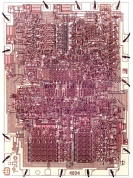
\includegraphics[angle=90,width=0.66\textwidth]{4004.pdf}
 \end{textblock*}
\end{frame}

\begin{frame}{Y UNIX ya había llegado en 1969}
  \begin{textblock*}{.63\textwidth}(0.4cm,1.2cm)
   \centering 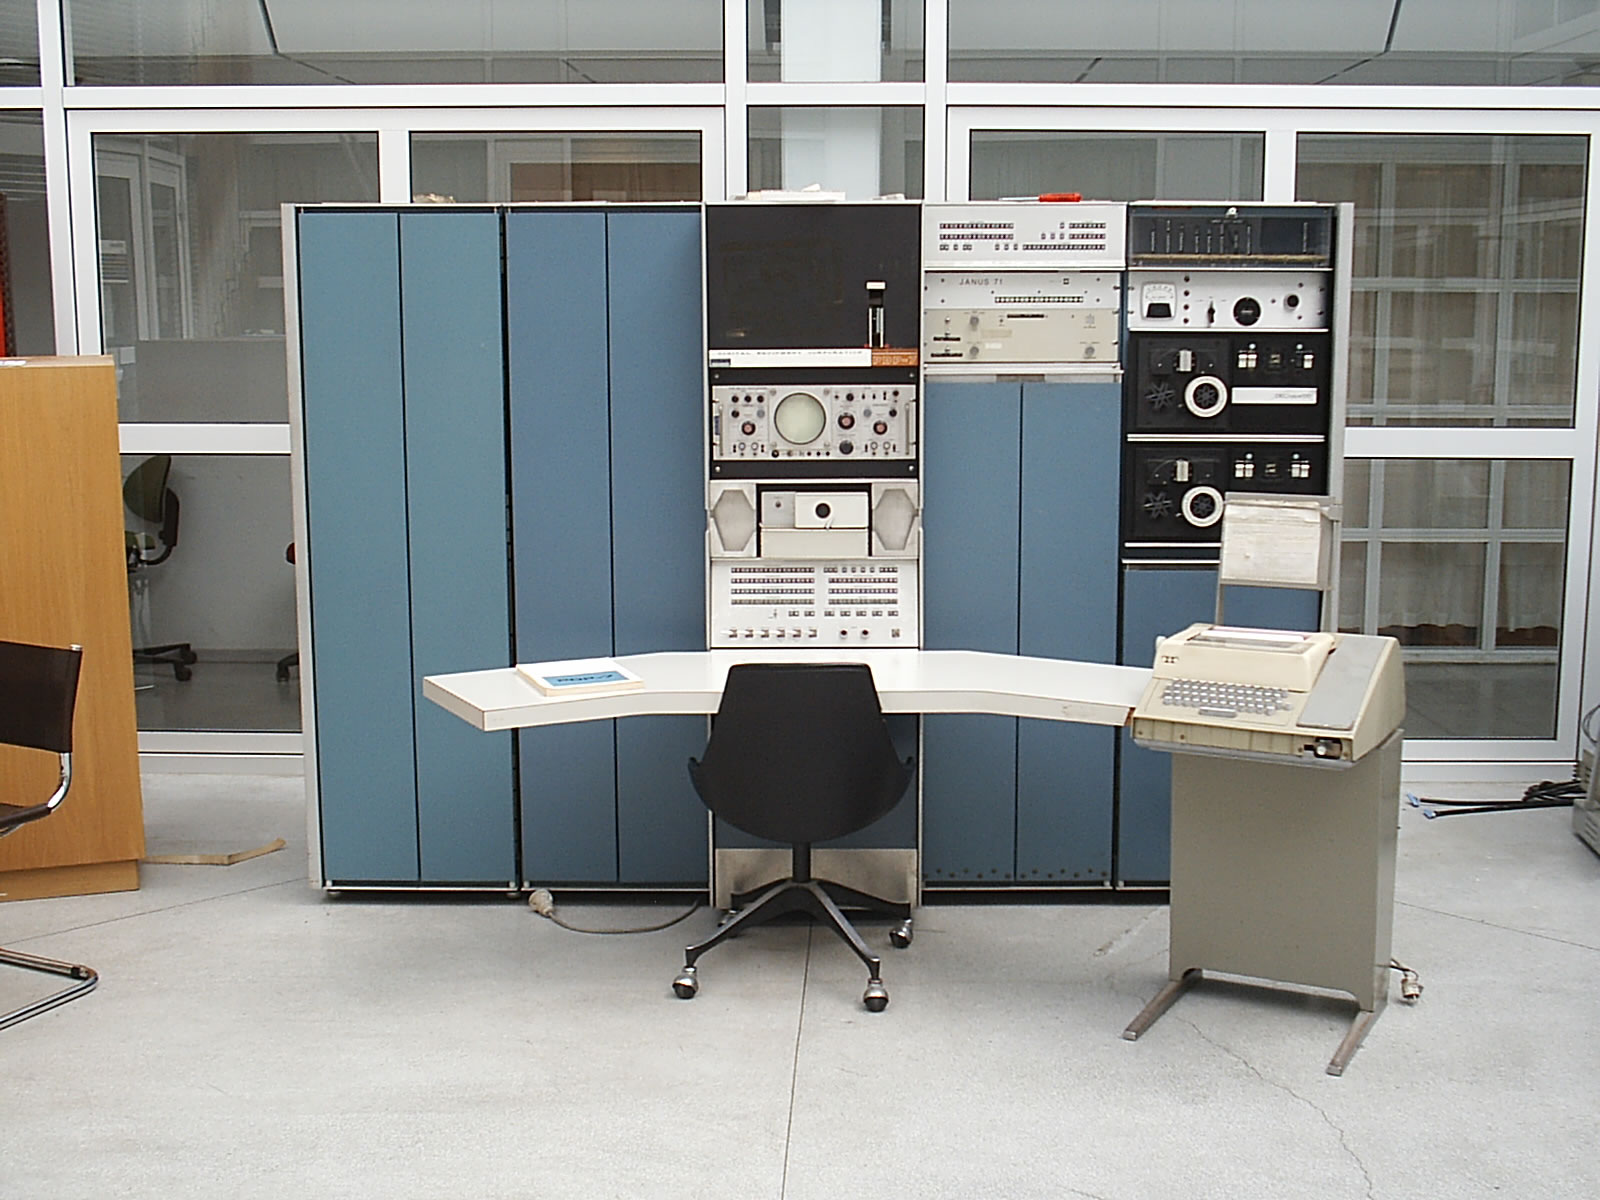
\includegraphics[width=\textwidth]{PDP-11.jpg}\\
  \end{textblock*}
  \begin{textblock*}{.36\textwidth}(.65\textwidth,1.2cm)
   \begin{itemize}[<+(1)->]\justifying
   \small
    \item La primera versión demo se\\
    desarrolló en una DEC PDP-7\\
    íntegramente en Assembler.
    \item La figura muestra una\\ DEC PDP-11. 
    \item A esta máquina se portó la\\
    primer versión de UNIX\\ escrita en C en 1970.
    \item Contaba con \SI{16}{\kibi\byte} de RAM\\
    y \SI{512}{\kibi\byte} de almacenamiento\dots
    \item \textcolor{furfiGreen}{No comprendo el motivo de\\
    esa sonrisa socarrona que\\
    tienen todos\dots}
   \end{itemize}
 \end{textblock*}
 \end{frame}

 \begin{frame}{La Ley de Moore}
  \begin{textblock*}{\textwidth}(0.4cm,1.15cm)
   \begin{itemize}[<+(1)->] \justifying
    \item El desarrollo de la tecnología de integración evolucionó de acuerdo con la predicción de Gordon Moore:\\
    \begin{center}
    \textcolor{furfiGreen}{\textit{``el número de transistores por unidad de superficie en circuitos integrados se\\
    duplica cada 2 años tendencia que continuará durante las siguientes décadas.''}}
    \end{center}
    \item Desde 2018 aproximadamente se han alcanzado dimensiones físicas de niveles\\
    atómicos para construir un transistor MOSFET, de modo que ya no es posible\\
    reducir mucho más las dimensiones de una compuerta.
    \item \textcolor{furfiBlue}{Estamos presenciando el fin de esta etapa. El futuro de la industria está abierto.}
    \vspace{0.3cm}
    \item Alrededor de 1980 se comienza a hablar de Circuitos Integrados VLSI\\
    (Very Large Scale Integration), en referencia a circuitos integrados que\\
    contienen cientos de miles de transistores integrados.
   \end{itemize}
  \end{textblock*}
 \end{frame}
 
\begin{frame}{Se empieza a acelerar la industria}
 \begin{textblock*}{\textwidth}(0.4cm,1.15cm)
  \begin{itemize}[<+(1)->]\justifying
   \item Con la tecnología SGT Intel lanza los procesadores 8008, 4040 y 8080,\\
   Motorola se plantea como competidor con su procesador 6800.
   \item Faggin plantea en Intel consolidar a la compañía como un fabricante de\\
   Microprocesadores. \textcolor{furfiBlue}{Noyce y fundamentalmente Gordon Moore\\
   no se deciden a abandonar el segmento de mercado de memorias.}
   \item \textcolor{furfiBlue}{En 1974 Faggin deja Intel y funda ZILOG.} En Marzo de 1976 lanza el Z80,\\
   que supera claramente al 8080 y al 8085 con el que Intel intentará contrarrestarlo,\\
   y por supuesto al 6800.
   \item Primeros computadores personales. Altair, Commodore, Sinclair, MSX, etc.\\
   utilizaron procesadores de \SI{8}{\bit}, \textcolor{furfiBlue}{particularmente el Z80, que se transforma\\
   en el procesador más empleado.}
   \item No era para menos. El Z80 era compatible con el 8080 (Faggin lo conocía a la\\
   perfección, obviamente), y además lo reforzaba con las instrucciones de manejo de\\
   bits propias del 6800, \textcolor{furfiBlue}{combinando en un solo procesador lo mejor de los dos mundos}.
  \end{itemize}
 \end{textblock*}
\end{frame}

\begin{frame}{El efecto Z80}
 \begin{textblock*}{\textwidth}(0.4cm,1.15cm)
  \begin{itemize} [<+(1)->] \justifying \parskip 0.1cm
   \item En 1975 Intel ofrecía dos procesadores: 8008 y 8080. Ambos diseños de Faggin.
   \item \textcolor{furfiBlue}{Gordon Moore impulsó el proyecto de un procesador muy superior, dando origen\\
   en ese año al proyecto 8800, que derivaría en la arquitectura iAPX432.}
   \item El diseño fue pensado como una arquitectura pura de \SI{32}{\bit}, con el objetivo de ser\\
   la \textcolor{furfiBlue}{nave insignia} de Intel en las ofertas de procesadores en la década de 1980.
   \item Considerablemente más poderoso y complejo que el 8080, el diseño superaba\\
   ampliamente las posibilidades del proceso tecnológico existente {\small \textcolor{furfiGray}{(Al apurar su\\
   lanzamiento, que terminó lanzado en 1981, debió ser dividido en varios chips individuales.)}}
   \item El deadline para su lanzamiento chocó de frente con el Z80, que literalmente\\
   \textcolor{furfiBlue}{estaba barriendo del mercado} a la oferta de Intel.
   \item Como conclusión el proyecto 8800 no podía seguir \textcolor{furfiBlue}{si no se neutralizaba el\\
   avance del Z80} como arquitectura dominante.
  \end{itemize}
 \end{textblock*}
\end{frame}


\begin{frame}{La era de la PC}
 \begin{textblock*}{\textwidth}(0.4cm,1.15cm)
  \begin{itemize} [<+(1)->] \justifying
   \item Sin perjuicio de la continuidad del proyecto 8800 al que apostaba su liderazgo futuro,\\
   \textcolor{furfiBlue}{Intel reúne un equipo de emergencia para diseñar un procesador más acotado que el\\
   del proyecto 8800 pero superior al Z80.}
   \item Y en tan solo 52 semanas está listo un procesador planteado como una evolución del\\
   8080 pero extendido a una arquitectura completa de \SI{16}{\bit}\textsuperscript{1}.
   \item \textcolor{furfiBlue}{En 1978 presenta la familia iAPx86 de la mano de su nave insignia, el 8086.}
   \item Se compromete a mantener \textcolor{furfiGreen}{compatibilidad} ascendente en los modelos subsiguientes\\
   de procesadores para satisfacer esta  demanda.
   \item {\small \textcolor{furfiGray}{Esto fue uno de los motivos de la decisión de IBM de adoptar esta familia de procesadores\\
   como base para su PC, y que los Z80 estaban parcialmente financiados por Exxon,\\
   competidor directo de IBM.}} Sólo requirió una versión con un bus exterior de \SI{8}{\bit}.\\
   Y finalmente fué el 8088.
  \end{itemize}
  \only <3->{\footnotesize \textsuperscript{1} S.P.  Morse,  W.B.  Pohlman, and B.W. Ravenel, “The Intel 8086 Microprocessor: A 16-bit Evolution of the 8080,” Computer, vol.11, no. 6, 1978, pp. 18–27)}
 \end{textblock*}
\end{frame}

\begin{frame}{Un cisne negro}
 \begin{textblock*}{\textwidth}(0.4cm,1.15cm)
  \begin{itemize} [<+(1)->] \justifying
   \item La elección de IBM del 8086 {\small (o mejor dicho de su primo hermano 8088 con bus\\
   externo de \SI{8}{\bit})} como procesador de su primer computadora personal \textcolor{furfiBlue}{fue un\\
   primer impulso para Intel} que estaba sufriendo fuerte erosión a manos del Z80.
   \item Pero además, el forecast de venta de IBM eran 250.000 computadoras\\
   \textcolor{furfiBlue}{y terminó vendiendo mas de 100 millones}.
   \item Y así una arquitectura pensada a \textcolor{furfiBlue}{corto plazo} {\small (dicho no por mí sino por su autor \textsuperscript{2})}\\
   termina revolucionando la industria y evolucionando por más de 4 décadas.\\
   \textcolor{furfiBlue}{Con Uds. el cisne negro.}
   \item En los 80 estamos en esta etapa. Aparecen Microsoft y Apple como actores nuevos\\
   de esta historia. \textcolor{furfiBlue}{El MS DOS se impone como Sistema Operativo y dominaría\\ la década del 80.}
  \end{itemize}
  \only<4->{\footnotesize \textsuperscript{2} The Intel 8086 Chip and the Future of Microprocessor Design. Stephen P. Morse. Computer , 50(4):8-9, 2017}
 \end{textblock*}
\end{frame}

\begin{frame}{Por si quedan dudas...}
 \begin{textblock*}{1.05\textwidth}(0.4cm,1.5cm)
 \shabox{
\textit{``Intel apostó su futuro a un procesador de alto desempeño, sin embargo, el diseño de dicho procesador llevaría años. 
Para contrarrestar a Zilog, Intel desarrolló un procesador temporal llamado 8086. 
Dicho procesador duraría muy poco tiempo en el mercado y no tendría sucesores, pero la historia no fue esa. 
El procesador de alto desempeño llegó tarde al mercado y era muy lento. 
De esta manera, el 8086 siguió en el mercado, y evolucionó a un procesador de 32 bits y eventualmente a 64 bits. 
Los nombres fueron cambiando (80186, 80286, i386, i486, Pentium), pero, por cuestiones de compatibilidad, 
el set de instrucciones permaneció intacto.''}
}

Stephen P. Morse, [Morse 2017]

 \end{textblock*}
\end{frame}

\begin{frame}{8086 Organización}
 \centering 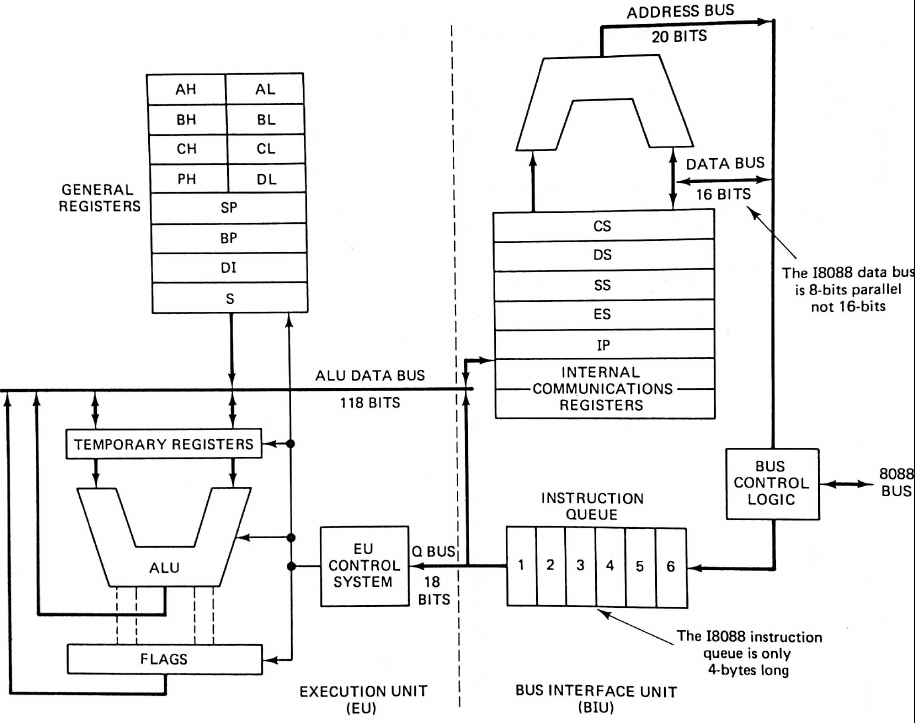
\includegraphics[width=0.6\textwidth]{8086-interno.png}
\end{frame}

\begin{frame}{Sistema básico de 8086}
 \centering 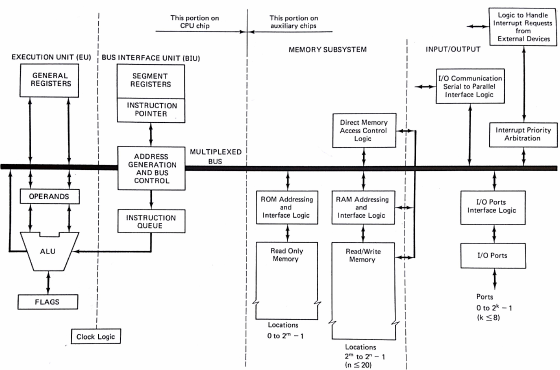
\includegraphics[width=0.7\textwidth]{8088-Sys.png}
\end{frame}

\begin{frame}{Familia iAPx86}
 \begin{textblock*}{\textwidth}(0.3cm,1.2cm)
  \begin{block}{Origenes}
   \justifying
   Unos meses luego del lanzamiento del 8086, primero procesador de la familia iAPx86\textsuperscript{3},
   Intel presenta a pedido de IBM \textcolor{furfiBlue}{una variante del mismo procesador}: el 8088, idéntico en
   su arquitectura interna de \SI{16}{\bit}, pero con un bus de datos externo de \SI{8}{\bit}, \textcolor{furfiBlue}{que permitía
   conectarle directamente la innumerable cantidad de periféricos} de \SI{16}{\bit} que por entonces había disponibles.
   Esto permitió a IBM lanzar su primer PC basada en un procesador 8088 (nunca usó el 8086).
  \end{block}
  \footnotesize \textsuperscript{3} \textbf{iAPX}, se reporta como la abreviación de \textbf{i}ntel \textbf{A}dvanced \textbf{P}rocessor ar\textbf{ch}itecture, la \textbf{X} proviene de la letra griega $\chi$ (\textbf{Ji} en castellano, \textbf{Chi} en inglés)
  \end{textblock*}
\end{frame}
 
\begin{frame}{Familia iAPx86}
 \begin{textblock*}{\textwidth}(0.3cm,1.2cm)
  \begin{block}{la primer prueba}
   \justifying
   En 1982 Intel presenta el 80286, que mejoraba la CPU 8086 en la ejecución de numerosas instrucciones e incorporó multitasking.
   \textcolor{furfiBlue}{Su arquitectura de \SI{16}{\bit} seguía siendo la misma}, y guardaba compatibilidad a nivel binario con el 8088
   (esto es, no hace falta recompilar los programas existentes). \textcolor{furfiBlue}{A partir de este procesador IBM diseña el modelo de PC conocido como AT.}
  \end{block}
  \end{textblock*}
\end{frame}
 
\begin{frame}{Familia iAPx86}
 \begin{textblock*}{\textwidth}(0.4cm,1.2cm)
  \begin{block}{La consolidación en \SI{32}{\bit}}
   \begin{itemize}[<+(1)->]\justifying
    \item En 1984 Intel \textcolor{furfiBlue}{extiende la arquitectura iAPx86 a \SI{32}{\bit}}. Lanza el 80386, y con él la arquitectura que denominará IA-32.
    \item La industria comienza a hablar de los procesadores x86, \textcolor{furfiBlue}{que en ese momento constituyen un standard}. (Es el fin del sueño iAPx432)
    \item La demanda de equipos de computo personal es astronómica \textcolor{furfiBlue}{superando la capacidad de Intel para abastecer al mercado}.
    \item Intel \textcolor{furfiBlue}{habilita a terceros la producción de procesadores IA-32} bajo licencia, para mantener el impulso de expansión de IA-32.
    \item Nace AMD.
    \item En los '90 Intel presenta el procesador Pentium y \textcolor{furfiBlue}{deja de habilitar a terceros su producción} bajo licencia. Nace el lema ``Intel Inside''.
   \end{itemize}
  \end{block}
 \end{textblock*}
\end{frame}
 
\begin{frame}{Aquel proyecto de 52 semanas lleva reinando más de dos décadas!}
 \begin{textblock*}{\textwidth}(0.4cm,1.2cm)
  \begin{block}{EPIC}
   \begin{itemize}[<+(1)->]\justifying
    \item A fines de los '90 Intel y Hewlett Packard desarrollan una arquitectura de \SI{64}{\bit}.
    \item Se basó en un concepto surgido como \textcolor{furfiBlue}{evolución del modelo \textbf{VLIW}}\\
    (\textbf{V}ery \textbf{L}arge \textbf{I}nstruction \textbf{W}ord)
    \item \textbf{E}xplicitly \textbf{P}arallell \textbf{I}nstruction \textbf{C}omputer (\textbf{EPIC}).
    \item \textcolor{furfiBlue}{El paralelismo de instrucciones lo resuelve el compilador} y el hardware se\\
    dedica a proveer \textcolor{furfiBlue}{fuerza bruta} de ejecución.\\
    \textcolor{furfiGreen}{Novedoso pero nunca explorado comercialmente.}
    \item Se presenta bajo el paraguas IA-64.
    \item El procesador \textcolor{furfiBlue}{Itanium} es el primer producto.
    \item No podía ejecutar código x86, \textcolor{furfiBlue}{ni se comercializaba junto con el compilador.}
   \end{itemize}
  \end{block}
 \end{textblock*}
\end{frame}
 
\begin{frame}{¿Y que pasó con EPIC?}
 \begin{textblock*}{\textwidth}(0.4cm,1.2cm)
  \only<2->{
   \begin{block}{\Large ``EPIC Failure''\normalsize \textsuperscript{4}}
    \only<2->{\centering 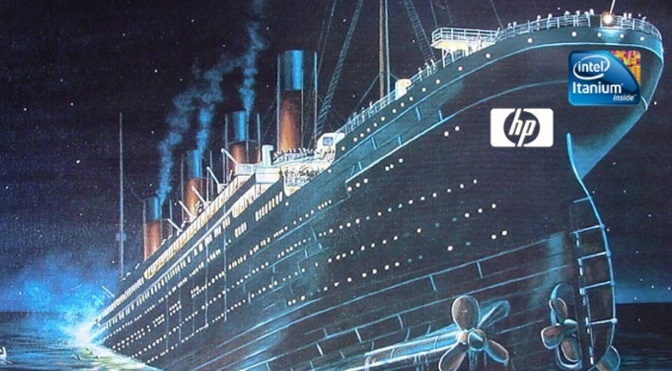
\includegraphics [width = 0.65 \textwidth ] {itanic.jpg}}
   \end{block}
   }
   \only<2->{\footnotesize \textsuperscript{4} \textit{``John Hennessy and David Patterson Deliver Turing Lecture at ISCA 2018''}}
 \end{textblock*}
\end{frame}

\begin{frame}{AMD toma su camino}
 \begin{textblock*}{\textwidth}(0.4cm,1.2cm)
  \begin{block}{Extiende IA-32 a \SI{64}{\bit}}
   \begin{itemize}[<+(1)->]\justifying
    \item Mientras Intel se embarcaba en el \textit{``itanic''} en busca de una arquitectura de \SI{64}{\bit},\\
    \textcolor{furfiBlue}{AMD toma IA-32 y la extiende a \SI{64}{\bit}.}
    \item Denomina a esta arquitectura AMD-64.
    \item \textcolor{furfiBlue}{Y las protege con una patente.}
    \item Nace el procesador Opteron, \textcolor{furfiBlue}{muy competitivo para Itanium} tanto en costo como\\
    en compatibilidad con IA-32
    \item AMD-64 tiene un submodo llamado compatibilidad que permite \textcolor{furfiBlue}{ejecutar código\\
    IA-32 nativo sin recompilar}.
   \end{itemize}
  \end{block}
 \end{textblock*}
\end{frame}

\subsection{Nace un paradigma de Arquitectura: RISC}
\begin{frame}{Orígenes de RISC}
 \begin{textblock*}{\textwidth}(0.4cm,1.2cm)
  \begin{itemize}[<+(1)->]\justifying \parskip 0.2cm
   \item Antes de las Personal Computers, \textcolor{furfiBlue}{el mercado era dominado por los denominados mainframes}.
   \item Los players eran IBM, Digital Electronic Corporation (DEC), Amdahl, entre otros.\\
   \textcolor{furfiBlue}{Sus computadores hoy son piezas de museo.}
   \item Sobre los años 80 aparecen los primeros microprocesadores de 16 bits con ciertas\\
   capacidades para hacer frente a una nueva generación de equipos de cómputo:
   \begin{itemize}
    \item Intel evoluciona el 8086/88 al 80286, y ensaya el iAPx432 citado como micromainframe processor, especialmente diseñado para ejecutar lenguajes de alto nivel como Ada.
    \item Motorola evoluciona el 68000 (citado como m68k)
   \end{itemize}
   \item Vimos que tienen todos un punto en común:\\
   \begin{center}
    \textcolor{furfiBlue}{Set de instrucciones de complejidad creciente}
   \end{center}
  \end{itemize}
 \end{textblock*}
\end{frame}

\begin{frame}{Orígenes de RISC}
 \begin{textblock*}{\textwidth}(0.4cm,1.0cm)
  \begin{block}{Líneas de Investigación}
   \justifying
   Durante los años '60 y '70, IBM, Control Data Corporation (CDC), y Data General (DG),
   incursionaron líneas de investigación tendientes a implementar procesadores con pocas
   instrucciones simples.

   En los '80 David Patterson\footnote[frame]{\tiny{David A. Patterson, Carlo H. Sequin. RISC I: A Reduced Instruction Set VLSI Computer}} \footnote[frame]{\tiny{David A. Patterson, David R. Ditzel. The case for the reduced instruction set computer}}  (Universidad de Berkeley), y John Hennesy\footnote[frame]{\tiny{Hennessy, J.L., Jouppi, N., Baskett, F., Gill, J. MIPS: A VLSI Processor Architecture. In Proceedings CMU Conference on VLSI Systems and Computations. Computer Science Press, October 1981}} (Universidad de Stanford) publicaron los primeros trabajos con resultados concretos, que presentaban una arquitectura contrapuesta con la de los Computadores que en ese momento dominaban la industria.\\
   \bigskip
   \textcolor{furfiBlue}{La denominaron \textbf{RISC} (\textbf{R}educed \textbf{I}nstruction \textbf{S}et \textbf{C}omputer).} Y esto motivó que a los procesadores diseñados hasta entonces se los etiquetar como \textbf{CISC}
  (Por \textbf{C}omplex \textbf{I}nstrucion \textbf{S}et \textbf{C}omputer)
  \end{block}
 \end{textblock*}
\end{frame}

\begin{frame}{¿Porque RISC?}
 \begin{textblock*}{.35\textwidth}(0.3cm,1.2cm)
  \centering 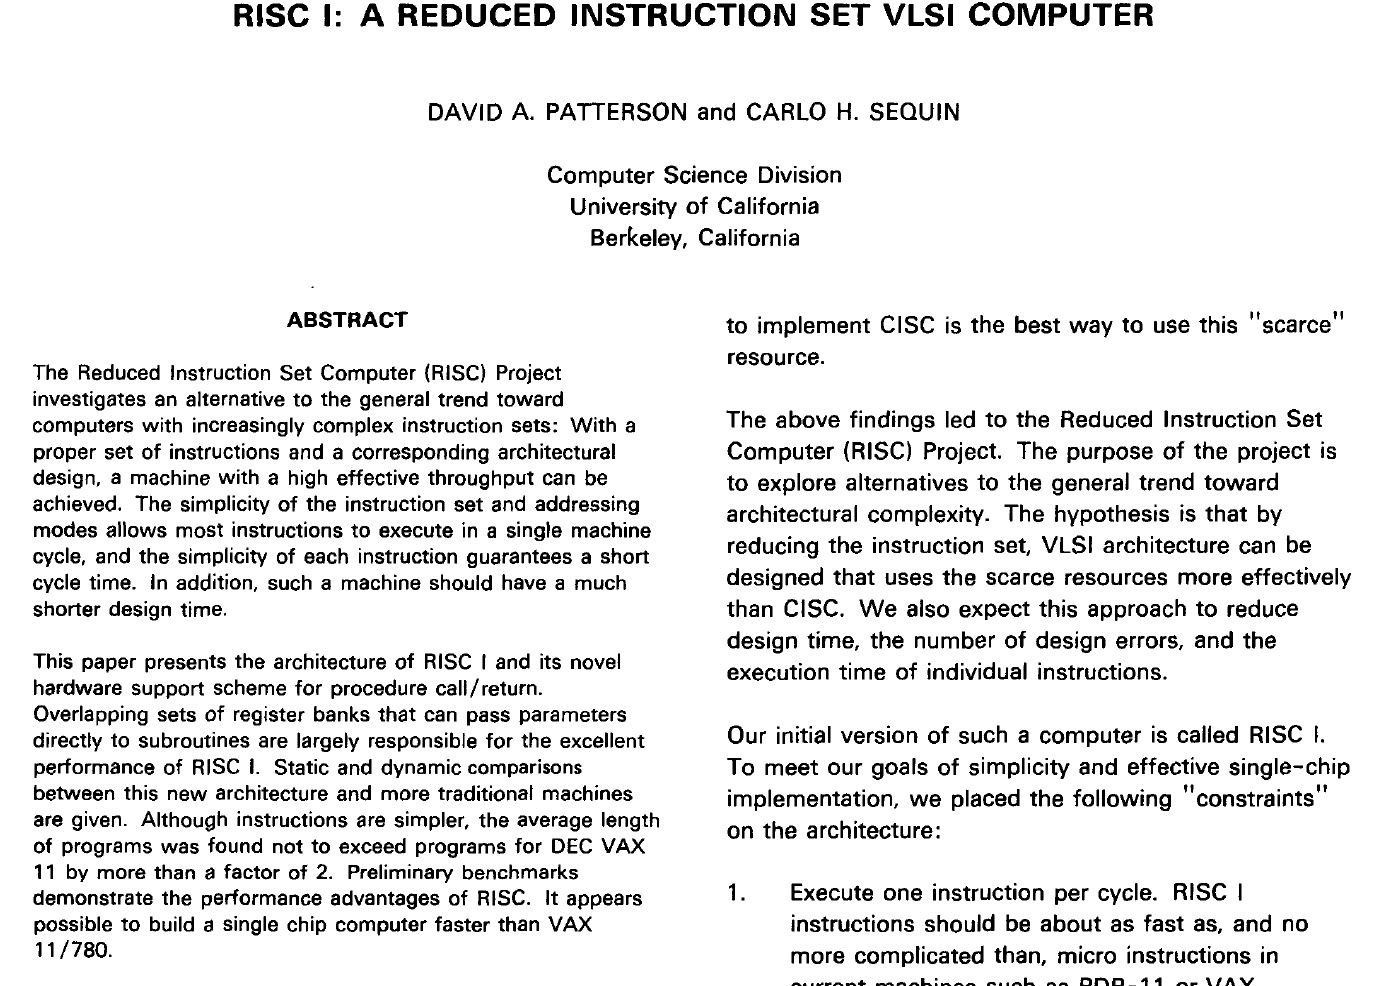
\includegraphics[width=\textwidth,angle=30]{PaperPaterson-1.png}
 \end{textblock*}
 \begin{textblock*}{.35\textwidth}(0.6\textwidth,1.2cm)
  \centering 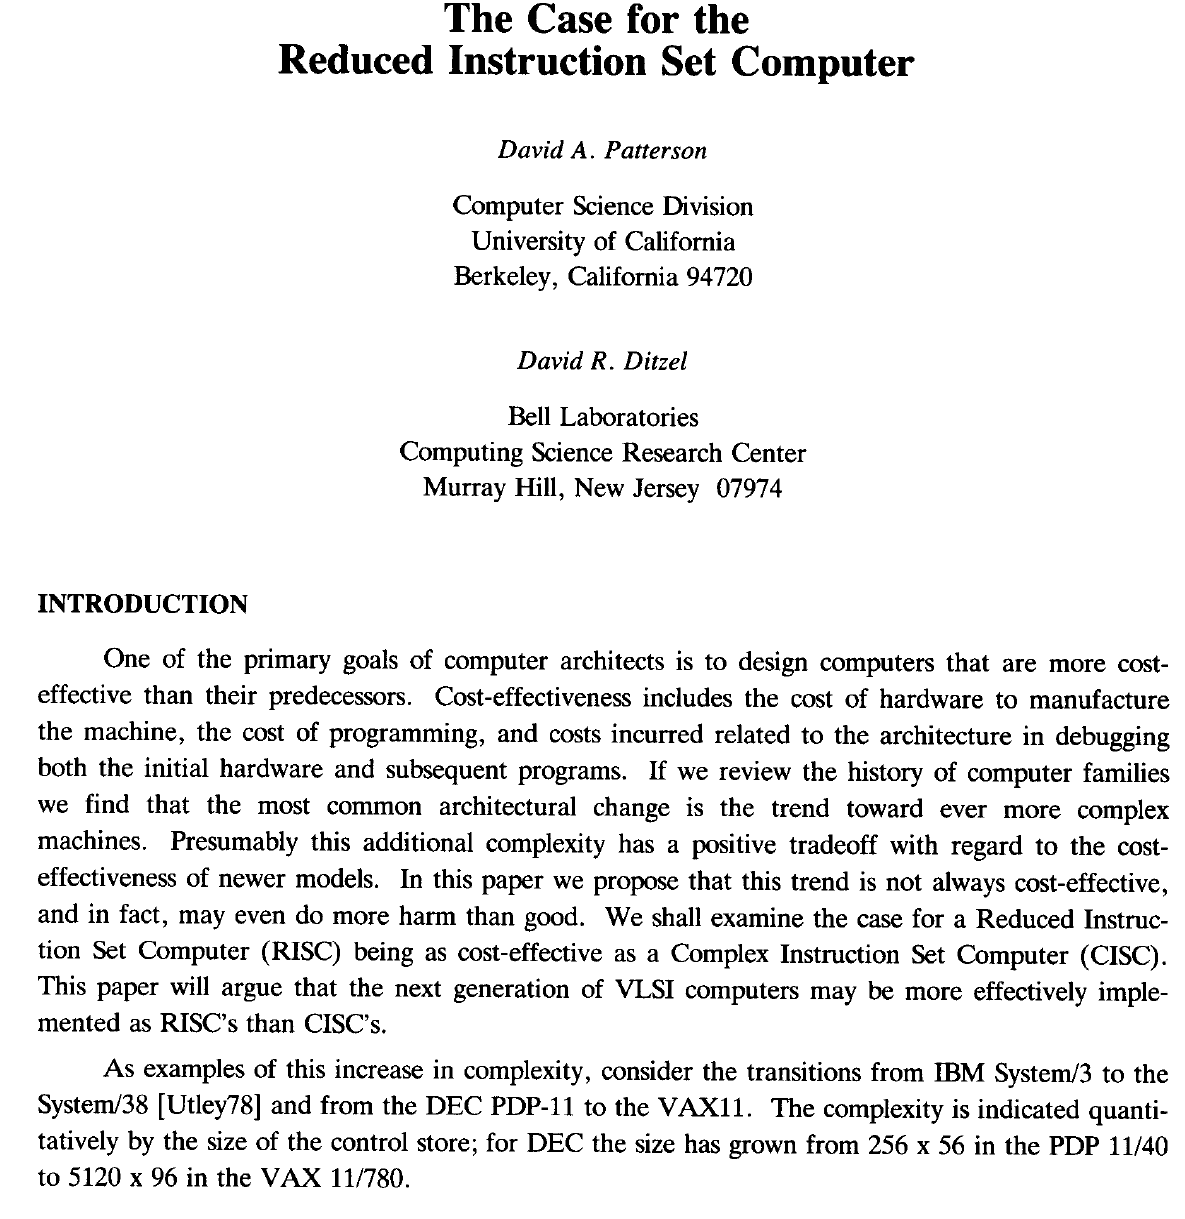
\includegraphics[width=\textwidth,angle=-30]{PaperPaterson-2.png}
 \end{textblock*}
 \begin{textblock*}{.4\textwidth}(0.3\textwidth,4.7cm)
  \centering 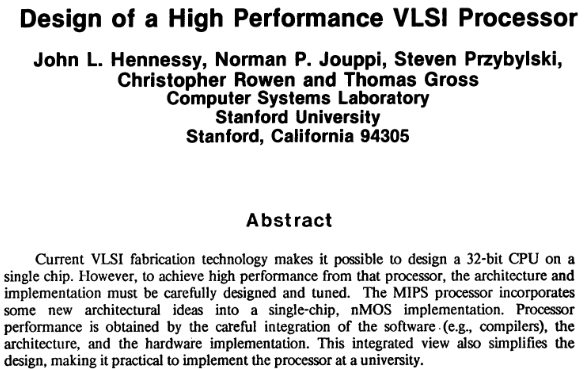
\includegraphics[width=\textwidth]{PaperHennesy.png}
 \end{textblock*}
\end{frame}

 %  \begin{frame}{Relación con el pipeline}
 %   \begin{textblock*}{\textwidth}(0.3cm,1.2cm)
 %    \begin{itemize}[<+(1)->]\justifying \parskip 0.2cm¸
 %     \item Se analizaron los obstáculos en un pipeline.
 %     \item En particular los obstáculos de datos impactan cuando involucran accesos a memoria para buscar operandos.
 %     \item Claramente si se evita que los operandos se accedan en memoria, en lugar de cargarlos previamente en un registro tal vez el pipeline pueda mejorarse.
 %     \item Otro aspecto es cuando demora la ejecución de las instrucciones mas complejas. En los diagramas teóricos hemos considerado un clock para ejecución, pero hay instrucciones que no pueden satisfacer este requisito. Éstas frenarían al Pipeline.
 %    \end{itemize}
 %   \end{textblock*}
 %  \end{frame}
 %
 % \begin{frame}[t]{Hennesy \& Patterson}
 %  \includegraphics[width=\textwidth]{XavierDavidMagneto.jpeg}
 % \end{frame}

\begin{frame}{Los Mandamientos RISC}
 \begin{textblock*}{\textwidth}(0.3cm,1.2cm)
  \begin{enumerate}[<+(1)->]\justifying \parskip 0.2cm
   \item Se dispone de un \textcolor{furfiBlue}{juego de registros numeroso}, todos de propósito general.
   \item Las instrucciones \textcolor{furfiBlue}{se ejecutan en un solo ciclo} de clock.
   \item Las instrucciones derivan en \textcolor{furfiBlue}{códigos de operación de igual formato y tamaño}.
   \item Las instrucciones deben ser \textcolor{furfiBlue}{sencillas de decodificar}.
   {\small Los números de registros se deben tener la misma ubicación en los códigos de la instrucción y deben requerir la misma cantidad de bits para su decodificación.}
   \item \textcolor{furfiBlue}{No se utiliza microcódigo} para decodificar instrucciones {\small (no hay instrucciones complejas, como DIV o MUL).}
   \item Los datos en memoria se acceden mediante \textcolor{furfiBlue}{instrucciones simples de transferencia}: LOAD y STORE.
  \end{enumerate}
 \end{textblock*}
\end{frame}

\begin{frame}[fragile]{Corolario}
 \begin{textblock*}{\textwidth}(0.3cm,1.2cm)
  \begin{enumerate}[<+(1)->]\justifying \parskip 0.2cm
   \item La \textcolor{furfiBlue}{verificación de una máquina RISC es mucho más simple de realizar}, y también es menor la probabilidad de liberar al mercado un procesador con defectos de lógica \textcolor{furfiBlue}{(Recordemos el bug de división del Pentium$@$90Mhz)}.
   \item Es esperable que el \textcolor{furfiBlue}{tamaño de los programas sea mayor}, debido a que lo que los procesadores CISC resuelven con microcódigo, los RISC lo resuelven en el software.\\
   Una multiplicación se resuelve siempre por acumulación de sumas.\\
   \centering $\displaystyle A*B = \sum_{i=1}^{A} \; B$
   \begin{itemize}
    \item En microcódigo se implementa la instrucción MUL.
    \item Por software se implementa con una subrutina.
   \end{itemize}
  \end{enumerate}
 \end{textblock*}
 \begin{textblock*}{0.29\textwidth}(10.7cm,5.1cm)
  \begin{onlyenv}<5->
   \begin{block}{Listado 2}
 \lstset{basicstyle=\footnotesize}
    \begin{lstlisting}
 ; R1 = R1 * R2
 otro:   add R1,R1,R1
         sub R2,R2,#1
         bne otro
     \end{lstlisting}
   \end{block}
  \end{onlyenv}
 \end{textblock*}
\end{frame}
  
\begin{frame}{Sentido de esta reseña}
 \begin{textblock*}{\textwidth}(0.3cm,1.2cm)
  \begin{itemize}[<+->]\justifying
   \item Durante la relativamente \textcolor{furfiBlue}{breve} historia de esta industria, la memoria fue desde el inicio, y durante muchas décadas el recurso mas escaso 
   {\small (en rigor sigue vigente la máxima de Von Neumann \textit{``la cantidad de memoria siempre será insuficiente''}).}
   \item Como hemos visto, en los albores esta escasez fue dramática. \SI{16}{\kibi\byte} de RAM (8 para el sistema operativo y 8 para las aplicaciones) en 1969,\dots huelgan las palabras.
   \item \textcolor{furfiBlue}{Actualmente, la memoria ha dejado de ser el principal problema ya que la tecnología de integración ha dado respuestas.}
   \item La preocupación central en estos días es sin lugar a dudas el \textcolor{furfiBlue}{consumo de energía eléctrica}. Basta leer las publicaciones científicas. 
   Un alto porcentaje de los trabajos científicos propone mejoras para lograr CI que consuman menor cantidad de energía para la misma tarea (es decir menor trabajo).
   \item En algún tiempo más esta situación estará superada. \textcolor{furfiBlue}{Y habrá nuevas restricciones.}
   \item \textcolor{furfiGreen}{En cada época los arquitectos de computadores lidiaron con restricciones y sus decisiones siempre son producto de éstas.}
  \end{itemize}
 \end{textblock*}
\end{frame}

%%%%%%%%%%%%%%%%%%%%%%%%%%%%%%%%
\section{Arquitectura y Organización}
\subsection{Introducción}

\begin{frame}{Arquitectura vs Microarquitectura}
 \begin{textblock*}{\textwidth}(0.3cm,1.2cm)
  \begin{itemize}[<+->]\justifying \parskip 0.2cm
  \item \textcolor{furfiBlue}{\textbf{Arquitectura}}\\
  Es el conjunto de \textcolor{furfiBlue}{recursos accesibles para el programador}, que por lo general\\
  se mantienen a lo largo de los diferentes modelos de procesadores de esa\\
  arquitectura {\small (puede evolucionar pero la tendencia es mantener compatibilidad hacia modelos anteriores)}.
  \begin{itemize}
    \item[-] Registros
    \item[-] Set de instrucciones
    \item[-] Estructuras de memoria relacionadas (descriptores de página p. ej.)
  \end{itemize}
  \item \textcolor{furfiBlue}{\textbf{Micro Arquitectura}}\\
  Es la \textcolor{furfiBlue}{implementación de la arquitectura}. El diseño lógico detrás del set de registros\\
  y del modelo de programación. Puede ser muy simple o sumamente robusta y\\
  poderosa. Cambia de un modelo a otro dentro de una misma familia.
  \end{itemize}
 \end{textblock*}
\end{frame}

\begin{frame}{Definición de la Arquitectura de un Computador}
 \begin{textblock*}{\textwidth}(0.3cm,1.2cm)
  \begin{itemize}[<+->]\justifying \parskip 0.3cm
   \item Se trata de definir los \textcolor{furfiBlue}{aspectos más relevantes} en la arquitectura de un computador procurando maximizar el rendimiento del procesador, pero sin dejar de satisfacer \textcolor{furfiBlue}{otras limitaciones impuestas} por los usuarios, como un costo accesible, o un consumo de energía moderado, entre otros.
   \item Requiere diseñar el \textcolor{furfiBlue}{set de instrucciones}, el \textcolor{furfiBlue}{modo en que se manejará la memoria} y sus \textcolor{furfiBlue}{modos de direccionamiento}, los restantes bloques funcionales que componen el CPU, como el \textcolor{furfiBlue}{File Register}, el \textcolor{furfiBlue}{DataPath} y el diseño de la \textcolor{furfiBlue}{lógica de control}.
   \item La implementación comprende \textcolor{furfiBlue}{el diseño del circuito integrado}, su encapsulado, montaje, alimentación y refrigeración.
  \end{itemize}
 \end{textblock*}
\end{frame}

% \subsection{Instruction Set Architecture (ISA)}
\begin{frame}{Definción de la ISA}
 \begin{textblock*}{\textwidth}(0.3cm,1.2cm)
  \justifying Nos referimos a \textit{\color{blue}Instruction Set Architecture}, como el set de instrucciones visibles por el programador. Es además el límite entre el software y el hardware.
  \begin{itemize}[<+->] \justifying \parskip 0.1cm
  \small
   \item \textbf{\color{blue}Clases de ISA.} ISAs con Registros de Propósito general vs. Registros dedicados. ISAs registro-memoria vs. ISAs Load Store.
   \item \textbf{\color{blue}Direccionamiento de Memoria.} Alineación obligatoria de datos vs. administración de a bytes.
   \item \textbf{\color{blue}Modos de Direccionamiento.} Como se especifican los operandos.
   \item \textbf{\color{blue}Tipos y tamaños de operandos.} Enteros, Punto Flotante, Punto Fijo.Diferentes tamaños y precisiones.
   \item \textbf{\color{blue}Operaciones}. Pocas Simples (RISC) o Muchas Complejas (CISC).
   \item \textbf{\color{blue}Instrucciones de control de flujo} Saltos condicionales, calls.
   \item \textbf{\color{blue}Longitud del código} Instrucciones de tamaño fijo vs. variable.
  \end{itemize}
 \end{textblock*}
\end{frame}

% \subsection{Organización y Hardware}
\begin{frame}{Microarquitectura = Organización + Hardware}
 \begin{textblock*}{\textwidth}(0.3cm,1.2cm)
  \begin{block}{Organización} \justifying
   Se refiere a los detalles de \textcolor{furfiBlue}{implementación de la ISA}. Es decir:
   \vspace{0.1cm}
   \begin{itemize}[<+(1)->] \justifying \parskip 0.1cm
    \item Organización e interconexión de la memoria.
    \item Diseño de los diferentes bloques de la CPU y para implementar\\ el set de instrucciones.
    \item Implementación de paralelismo a nivel de Instrucciones, y/o de datos.
    \item Podemos así encontrar procesadores que poseen la misma ISA pero una\\ organización muy diferente.
   \end{itemize}
  \end{block}
  \uncover<6->{
   \begin{block}{Ejemplo:} \justifying
    Los procesadores AMD FX y los Intel Core i7, tienen la misma ISA, sin embargo organizan su caché y su motor de ejecución de maneras diferentes.
   \end{block}
  }
 \end{textblock*}
\end{frame}

\begin{frame}{Microarquitectura = Organización + Hardware}
 \begin{textblock*}{\textwidth}(0.3cm,1.2cm)
  \begin{block}{Hardware}
   \begin{itemize}[<+(1)->]\justifying
    \item Se refiere a los \textcolor{furfiBlue}{detalles de diseño lógico} y \textcolor{furfiBlue}{tecnología de fabricación}.
    \item Existirán por lo tanto, \textcolor{furfiBlue}{procesadores con la misma ISA y la misma organización},\\
    pero absolutamente distintos a nivel de hardware y diseño lógico detallado.
   \end{itemize}
  \end{block}
  \vspace{0.3cm}
  \only<4->{
   \begin{block}{Ejemplo:} \justifying
    El Pentium 4, diseñado para desktop, y el Pentium 4 M para notebooks. Este último tiene una cantidad de lógica para control del consumo de energía, siendo su hardware muy diferente del del Pentium 4 desktop.
   \end{block}
  }
 \end{textblock*}
\end{frame}

\begin{frame}{¿Porque necesitamos saber todo esto?}
 \begin{textblock*}{\textwidth}(0.3cm,1.2cm)
  \begin{itemize}[<+(1)->] \justifying \parskip 0.5cm
   \item Para comprender \textcolor{furfiBlue}{lo que ocurre debajo del software}.
   \item Comprender como los diseños de hardware \textcolor{furfiBlue}{impactan en el software} y en el programador.
   \item Estar en condiciones de cruzar verticalmente las capas que \textcolor{furfiBlue}{separan el silicio} de la aplicación.
   \item Comprender las nociones básicas que \textcolor{furfiBlue}{rigen el diseño de un sistema} de cómputo moderno.
  \end{itemize}
 \end{textblock*}
\end{frame}

%%%%%%%%%%%%%%%%%%%%%%%%%%%%%%%%%%
\section{Implementando la arquitectura}
\subsection{El Procesador}
\begin{frame}{Datapath, Unidades de Cálculo, y Control}
 \begin{textblock*}{\textwidth}(0.3cm,1.1cm)
  \begin{itemize}[<+(1)->]\justifying
   \item Sea cual sea el set de instrucciones que se vaya a implementar, \textcolor{furfiBlue}{hay dos actividades que inicialmente cualquier instrucción debe realizar}:
   \begin{enumerate}\justifying
    \item Apuntar el Program Counter (\textbf{PC}) a la posición de memoria que contiene la siguiente instrucción.
    \item Leer uno o dos registros (dependiendo de la instrucción) contenidos en la palabra de instrucción. Ej: \textbf{\texttt{ld}} o \textbf{\texttt{lw}} requieren leer solo un registro: el que contiene la dirección de memoria que hay que leer. Otros tipos de instrucción leen dos registros.
   \end{enumerate}
   \item Las acciones posteriores del procesador dependen de cada \textcolor{furfiBlue}{instrucción específica}.
   \item No obstante cuanto \textcolor{furfiBlue}{mas simple} sea el set de instrucciones (RISC), el paso siguiente será \textcolor{furfiBlue}{el mismo} para un porcentaje mayor de instrucciones.
   \item Luego de los dos pasos anteriores un porcentaje de instrucciones \textcolor{furfiBlue}{utiliza la ALU}.
   \item Las instrucciones de \textcolor{furfiBlue}{referencia a memoria} (load, store y branch incondicional), utilizan la ALU para calcular la dirección de memoria a acceder, las instrucciones artitméticas y lógicas utilizarán la ALU para ejecutar la instrucción solicitada, los \textcolor{furfiBlue}{saltos condicionales} para evaluar la condición del salto. 
  \end{itemize}
 \end{textblock*}
\end{frame}
 
\subsection{Implementación del Procesador}
\begin{frame}{Diseño de un DataPath Simple}
 \begin{textblock*}{.95\textwidth}(0cm,1.7cm)
  \centering 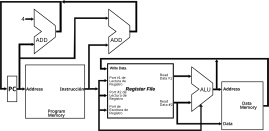
\includegraphics[width=0.9\textwidth]{Datapath-1.pdf}
 \end{textblock*}
 \begin{textblock*}{.5\textwidth}(.51\textwidth,1.5cm)
  \justifying \only<1>{\textcolor{furfiBlue}{El Datapath es el camino que recorren instrucciones y datos} por los buses internos y los bloques circuitales necesarios para su procesamiento.}
  \only<2->{Inicia en la \textcolor{furfiBlue}{memoria} cuando se busca una instrucción o cuando se busca un dato. 
  \textcolor{furfiBlue}{Afecta al \textbf{PC}}, que se debe ajustar a la siguiente instrucción.
  En este caso se le suma 4, en el primer sumador, ya que se asume un CPU RISC con tamaño de instrucción \SI{32}{\bit}}
 \end{textblock*}
\end{frame}

\begin{frame}{El Register File}
  \begin{itemize}[<+(1)->]\justifying
   \item Una estructura fundamental en el \textbf{Datapath} es el \textcolor{furfiBlue}{Register File}. 
   \item Un Register File de tamaño \textbf{n}, consiste en un \textcolor{furfiBlue}{arreglo de \textbf{n} registros}, numerados de \textbf{0} a \textbf{n-1}, que se pueden \textcolor{furfiBlue}{leer y escribir} proporcionando tan solo el número de registro al que se accede.
   \item \textcolor{furfiGray}{Se puede implementar con un decodificador para cada puerto de lectura o escritura y un arreglo de registros construida a partir de Flip-Flop's  D.}
   \item Dado que la \textcolor{furfiBlue}{lectura} de un registro no cambia ningún estado, y la salida Q de un FF está disponible, solo necesitamos proporcionar un número de registro como entrada, y la única salida serán los datos contenidos en ese registro. 
   \item Para \textcolor{furfiBlue}{escribir} un registro, necesitaremos tres entradas: el número de registro dentro del arreglo, los datos a escribir y un \textbf{clock} que controla la escritura en el registro.
   \item \textcolor{furfiBlue}{Utilizamos un Register File con dos puertos de lectura y uno de escritura.}\\
   Se muestra en el slide siguiente.
  \end{itemize}
\end{frame} 

\begin{frame}{El Register File}
 \begin{textblock*}{\textwidth}(0.4cm,1.6cm)
  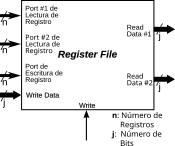
\includegraphics[width=.50\textwidth]{RegisterFile-Simbol.pdf}
 \end{textblock*}
 \begin{textblock*}{0.48\textwidth}(.53\textwidth,1.1cm)
  \begin{itemize}[<+(1)->]\justifying
   \item Se representa el símbolo de un Register File de \textbf{n}x\textbf{j} (\textbf{n} registros de \textbf{j}bit c/u).
   \item Para evitar atascos y agilizar el procesamiento es conveniente al menos dos puertos de lectura. 
   \item \textcolor{furfiBlue}{Puede leerse los dos operandos de una instrucción de una sola vez.}
   \item Un puerto es una entrada de \textbf{n} bits al que se envía el número de registro cuyo valor se desea leer.
   \item El contenido del registro sale por las \textbf{j} líneas \textbf{\texttt{Read Data \#1}} o \textbf{\texttt{Read Data \#2}} según el puerto seleccionado.
   \item Un solo puerto para escritura.
  \end{itemize}  
 \end{textblock*}
\end{frame}

\begin{frame}{El Register File en detalle}
 \begin{textblock*}{\textwidth}(0.3cm,1.3cm)
  \centering 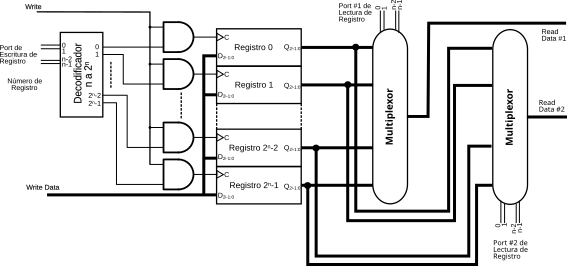
\includegraphics[width=\textwidth]{RegisterFile.pdf}
 \end{textblock*}
\end{frame}

\begin{frame}[fragile]{El Register File en Verilog (behavioral)}
 \begin{textblock*}{\textwidth}(0.4cm,1.15cm)
  \begin{lstlisting}[basicstyle=\scriptsize,language=Verilog,escapechar=|]
    reg [31:0] A;
    wire [31:0] b;
    
    always @(posedge clock) A<=b:

module registerfile (Read1, Read2, WriteReg, WriteData, RegWrite, Data1, Data2, clock);
    input[5:0] Read1, Read2, WriteReg; // Cant Registros a leer o escribir
    input[31:0] WriteData; // Puerto de escritura
    input RegWrite; //Control de escritura
    clock ; //L|\color{purple}\'i|nea de clock para disparar la escritura
    output[31:0] Data1, Data2; //Puertos de lectura de registros
    reg[31:0] RF[31:0] ; //32 Registros de 32 bits

    assign Data1 = RF[Read1];
    assign Data2 = RF[Read2];

    always begin
      //Escribir el nuevo valor en el registro si REgWrite es alto
      @(posedge clock) if (RegWrite) RF[WriteReg] <= WriteData
    end
endmodule 

  \end{lstlisting}
 \end{textblock*}
\end{frame}

\subsection{Pipeline}
\begin{frame}{Máquina de estados elemental}
 \begin{textblock*}{\textwidth}(0.4cm,1.5cm)
  \centering 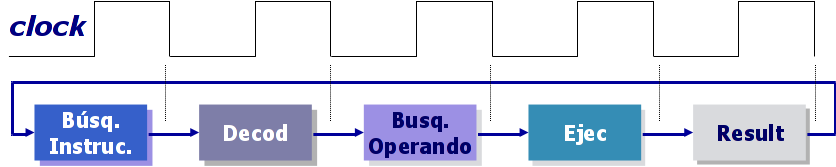
\includegraphics[width=\textwidth]{cicloInstruc.pdf}
  \vspace{-0.2cm}
  \begin{itemize}[<+(1)->]\justifying
   \item Un procesador \textcolor{furfiBlue}{ejecuta una máquina de estados} compuesta por diferentes etapas.
   \item En las primeras generaciones de microprocesadores cada etapa se ejecutaba durante uno o mas ciclos de clock, \textcolor{furfiBlue}{durante los cuales la CPU entera estaba dedicada a ella}.
   \item Una vez finalizada una etapa, en el siguiente ciclo de clock \textcolor{furfiBlue}{se pasaba a ejecutar la siguiente}.
   \item De este modo, ejecutar una instrucción \textcolor{furfiBlue}{insumía varios ciclos de clock}.
  \end{itemize}
 \end{textblock*}
\end{frame}

\begin{frame}{Pipelining}
 \begin{textblock*}{\textwidth}(0.3cm,1.2cm)
  \begin{tcolorbox}[enhanced jigsaw,rounded corners, drop fuzzy shadow=ShadowColor]
   Es una técnica de implementación que permite la ejecución simultánea de múltiples instrucciones, paralelizando por hardware las acciones necesarias para ejecutar una instrucción.

   \only<2->{Permite crear el efecto de \textcolor{furfiBlue}{superponer en el tiempo}, la ejecución de varias instrucciones a la vez.}

   \only<3->{Actualmente, el procesamiento paralelo es la técnica clave para la fabricación de procesadores rápidos. Un comodity. Incluso los procesadores que cuestan menos de un dólar utilizan algo de paralelismo.}
  \end{tcolorbox}
 \end{textblock*}
\end{frame}

\begin{frame}{Pipelining}
 \begin{textblock*}{\textwidth}(0.3cm,1.2cm)
  \begin{tcolorbox}[enhanced jigsaw,rounded corners, drop fuzzy shadow=ShadowColor]
   En una cadena de montaje de automóviles, donde existen numerosos pasos, cada uno de los cuales contribuye a la construcción de, por ejemplo, un vehículo.

   \only<2->{Cada paso opera en paralelo con los demás, \textit{\color{furfiBlue}aunque en un vehículo diferente}.}

   \only<3->{\textcolor{furfiBlue}{En un pipeline informático, cada paso completa una parte \textbf{de una instrucción diferente}}. Los distintos pasos completan diferentes partes de distintas instrucciones en paralelo.}

   \only<4->{\textcolor{furfiBlue}{Cada uno de estos pasos se denomina segmento o etapa (\textbf{stage}) del pipeline.}}
  \end{tcolorbox}
 \end{textblock*}
\end{frame}

\begin{frame}{Pipeline}
 \begin{textblock*}{\textwidth}(0.3cm,1.2cm)
  \begin{tcolorbox}[enhanced jigsaw,rounded corners, drop fuzzy shadow=ShadowColor]
   Las etapas se conectan entre sí para formar un pipeline: \textbf{\color{Blue}las instrucciones entran por un extremo, avanzan a través de las etapas y salen por el otro}, al igual que los vehículos en una cadena de montaje.
  \end{tcolorbox}
  \begin{itemize}[<+(1)->]\justifying
   \item Cada etapa completa una parte de una instrucción.
   \item Las distintas etapas completan en un mismo momento (de ahora en mas \textbf{\color{Blue}en paralelo}), diferentes partes de distintas instrucciones.
   \item El rendimiento de una línea de montaje es la frecuencia con la que cada elemento sale terminado.
   \item El rendimiento de un pipeline de instrucciones está determinado por la frecuencia con la que es capaz de enviar una instrucción a su salida.
   \item El tiempo necesario para que una instrucción avance un paso por el pipeline se denomina \textcolor{furfiBlue}{ciclo de procesador}.
  \end{itemize}
 \end{textblock*}
\end{frame}

\begin{frame}{Pipeline}
 \begin{textblock*}{\textwidth}(0.3cm,1.2cm)
  \begin{itemize}[<+->] \justifying
   \item Como todas las etapas se ejecutan al mismo tiempo, \textcolor{furfiBlue}{la duración de un ciclo de procesador está determinada por el tiempo que tarda la etapa más lenta}.
   \item En un computador, \textbf{\color{furfiGreen}un ciclo de procesador casi siempre dura un ciclo de reloj}.
   \item De este modo crea el efecto de superponer en el tiempo, la ejecución de varias instrucciones.
   \item Es el primer pequeño paso de lo que hoy denominamos \textit{\textbf{\color{blue}Instruction Level Paralelism (ILP)}}, dado a fines de los años 1970'.
   \item \textcolor{furfiBlue}{Requiere muy poco o ningún hardware adicional para interconectar las etapas.}
   \item Solo necesita que los bloques del procesador que resuelven la máquina de estados para la ejecución de una instrucción, operen en paralelo.
   \item Es decir, los bloques funcionales trabajan en paralelo pero cada uno en una instrucción diferente.
  \end{itemize}
 \end{textblock*}
\end{frame}

\begin{frame}{Pipeline}
 \begin{textblock*}{\textwidth}(0.3cm,1.2cm)
  \begin{itemize}[<+->] \justifying
   \item El objetivo del diseñador es equilibrar la duración de cada etapa.
   \item Si las etapas están perfectamente equilibradas, el tiempo por instrucción ($TPI_{p}$) en el procesador pipeline en condiciones ideales es igual a:
   \begin{center}
    $ TPI_{p}\: =\: \frac{Tiempo\: por\: instrucci\acute{o}n\: en\: la\: CPU\: " No-Pipeline\textquotedblright}{Cantidad\: de\: etapas} $
   \end{center}
   \item La aceleración \textbf{\color{Blue}ideal} que se logra con pipelining es igual al número de etapas (como una línea de montaje de \textit{n} etapas, \textbf{\color{Blue}idealmente}, produce autos \textit{n} veces más rápido.)
   \item Normalmente las etapas no están perfectamente equilibradas. Además, el hardware que interconecta cada etapa implica cierta sobrecarga. Por lo tanto, el tiempo por instrucción en un procesador pipeline no alcanza su valor mínimo posible (ideal).
   \item Pipelining reduce el tiempo medio de ejecución por instrucción.
   \item Si un procesador inicial tarda \textit{n} ciclos de reloj por instrucción, el pipeline reduce el CPI (ciclos por instrucción). Esta es la perspectiva principal que adoptaremos.
   \item A diferencia de algunas técnicas de aceleración, \textbf{\color{Blue}no es visible para el programador}.
  \end{itemize}
 \end{textblock*}
\end{frame}
%%%%%%%%%%%%%%%%%%%%%%%%%%
% \begin{frame}{Pipeline}
%   \begin{itemize}[<+->] \justifying
%    \item Permite crear el efecto de \textcolor{furfiBlue}{superponer en el tiempo}, la ejecución de varias instrucciones a la vez.
%    \item Formaliza el concepto de \textit{\textbf{\color{blue}Instruction Level Paralelism (ILP)}}.
%    \item \textcolor{furfiBlue}{Requiere muy poco o ningún hardware adicional}.
%    \item Solo necesita que los bloques del procesador que \textcolor{furfiBlue}{resuelven la máquina de estados} de ejecución de una instrucción, operen en forma simultánea.
%    \item \textcolor{furfiBlue}{Se logra si todos los bloques funcionales trabajan en paralelo, pero cada uno en una instrucción diferente.}
%    \item Es algo parecido al concepto de una \textcolor{furfiBlue}{línea de montaje}, en donde cada operación se descompone en partes, y se ejecutan en un mismo momento diferentes partes de diferentes operaciones.
%    \item \textcolor{furfiBlue}{Cada parte se denomina etapa (\textbf{stage})}
%   \end{itemize}
% \end{frame}

\begin{frame}{Versión de un Pipeline clásico}
 \begin{textblock*}{\textwidth}(0.3cm,1.2cm)
  \centering 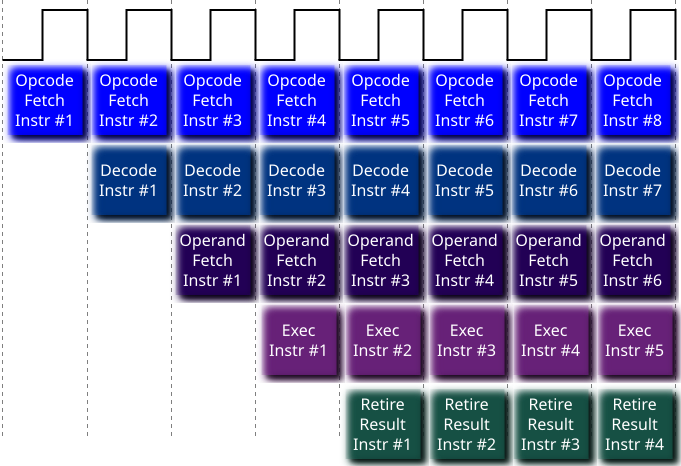
\includegraphics[width=0.6\textwidth]{pipeline.pdf}
 \end{textblock*}
 \begin{textblock*}{\textwidth}(0.3cm,7.3cm)
  \begin{block}{}
  \centering Este modelo es teórico y representa la situación ideal.
  \end{block}
 \end{textblock*}
\end{frame}

%%%%%%%%%%%%%%%%%%%%%

\begin{frame}{Pipeline clásico}
 \begin{block}{Conclusiones Preliminares}
  \begin{enumerate} [<+(1)->] \justifying \parskip 0.3cm
   \item El pipeline llega a su \textcolor{furfiBlue}{condición de régimen} luego de tantos ciclos de clock como etapas tenga.
   \item En un pipeline de 5 etapas, y en el \textcolor{furfiBlue}{caso ideal} en que cada etapa consuma solamente un ciclo de clock, una arquitectura pipeline provee un resultado de instrucción por cada ciclo de clock, a partir del ciclo de clock en el cual se llega a resolver la primer instrucción.
   \item Este escenario permanente es puramente teórico. \textcolor{furfiBlue}{En la práctica no se cumple todo el tiempo.}
  \end{enumerate}
 \end{block}
\end{frame}
 
\begin{frame}{Profundidad del Pipeline}
 \begin{textblock*}{\textwidth}(0.3cm,1.2cm)
  \begin{itemize}
   \item La expresión teórica anterior:
   \begin{center}
    $ TPI_{p}\: =\: \frac{Tiempo\: por\: instrucci\acute{o}n\: en\: la\: CPU\: " No-Pipeline\textquotedblright}{Cantidad\: de\: etapas} $
   \end{center}
   Induce a suponer que agregar etapas mejoraría la performance.
   \item Etapas mas simples aseguran que cumplan su función en un solo clock para cualquier instrucción.
   \item De este modo se aproxima al comportamiento ideal: \textcolor{Blue}{un ciclo de procesador dura un ciclo de reloj para cualquier instrucción}
   \item Por eso podríamos pensar en aumentarlas mas y mas $\dots$
  \end{itemize}
 \end{textblock*}
\end{frame}

\begin{frame}{Profundidad del Pipeline}
 \begin{textblock*}{\textwidth}(0.3cm,1.5cm)
  \centering 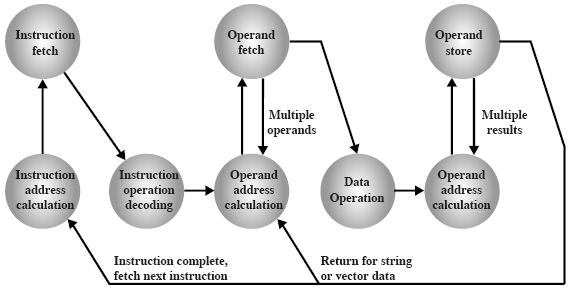
\includegraphics[width=.8\textwidth]{pipeline2.png}
 \end{textblock*}
\end{frame}

\begin{frame}{Mas y mas etapas...}
 \begin{textblock*}{\textwidth}(0.3cm,1.5cm)
  \centering 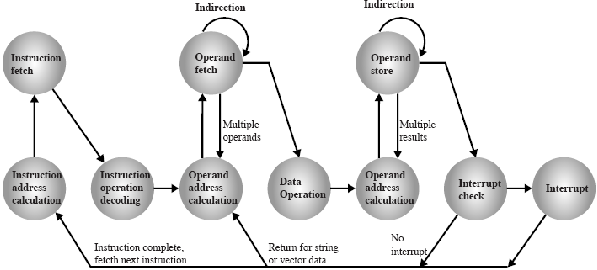
\includegraphics[width=0.8\textwidth]{pipeline3.png}
 \end{textblock*}
\end{frame}

\begin{frame}{Conclusiones}
 \begin{textblock*}{\textwidth}(0.3cm,1.2cm)
  \begin{itemize}[<+(1)->] \justifying
   \item La situación teórica e ideal dada por la ecuación anterior \textcolor{furfiBlue}{no es 100\% cierta}.
   \item En la práctica existen \textcolor{furfiBlue}{overheads introducidos por el hardware} de implementación del pipeline, que suman \textcolor{furfiBlue}{pequeñas demoras} en la interfaz entre cada una de sus etapas. La realidad es que si bien existen, estas demoras resultan suficientemente pequeñas como para aceptar que el \textbf{\textit{TPI}} así calculado, se aproxima mucho al ideal.
   \item El resultado es que el efecto del pipeline en la práctica se percibe en una cantidad de ciclos de clock significativamente menor para ejecutar cada instrucción.
   \item \textcolor{furfiBlue}{El pipeline no reduce el tiempo de ejecución de cada instrucción individual}, sino que al aplicarse en paralelo al flujo de instrucciones, incrementa el número de instrucciones completadas por unidad de tiempo.
   \item De hecho el \textcolor{furfiBlue}{overhead del pipeline} perjudica el tiempo de ejecución individual, aunque de manera poco significativa, al agregar un $\delta.t$ a cada instrucción.
   \item El rendimiento (throughput) del procesador \textcolor{furfiBlue}{mejora notablemente} ya que los programas ejecutan notablemente mas rápido.
  \end{itemize}
 \end{textblock*}
\end{frame}
 
\subsubsection{Riesgos en un pipeline}
\begin{frame}{Obstáculos de un pipeline}
 \begin{textblock*}{\textwidth}(0.3cm,1.2cm)
  \begin{itemize}[<+(1)->] \justifying \parskip 0.2cm
   \item Hay \textcolor{furfiBlue}{obstáculos} que conspiran contra la eficiencia de un pipeline.\\
   \item Podemos agruparlos en tres categorías:\\\
   \begin{enumerate}
    \item \textbf{\textit{\color{blue}Obstáculos estructurales}}.\\\
    \item \textbf{\textit{\color{blue}Obstáculos de datos}}.\\\
    \item \textbf{\textit{\color{blue}Obstáculos de control}}.\\\
   \end{enumerate}
   \item Al \textcolor{furfiBlue}{efecto ocasionado} por un obstácuo se lo denomina \textbf{\textit{\color{blue}pipeline stall}}.\\
   \item Su efecto degrada la performance del procesador.
  \end{itemize}
 \end{textblock*}
\end{frame}
 
\begin{frame}{Obstáculos Estructurales}
 \begin{textblock*}{\textwidth}(0.3cm,1.2cm)
  Se pueden dar por varias razones:
  \begin{itemize}[<+->] \justifying \parskip 0.3cm
   \item \textcolor{furfiBlue}{Una etapa no está suficientemente atomizada}, y concentra aún demasiadas funciones lo que hace que para completarse requiere mas de un ciclo de clock.
   \item Si dos instrucciones que utilizarán esta etapa están mas próximas del tiempo que necesita esta etapa para procesar su parte, \textcolor{furfiBlue}{caerán en conflicto de recursos para su ejecución}.
   \item Este grupo de instrucciones entonces, no puede pasar por esa etapa del pipeline en un ciclo de clock.
   \item En estas circunstancias \textcolor{furfiBlue}{una de las instrucciones debe detenerse}. Como consecuencia CPI se incrementa en 1 o mas respecto del valor ideal.
  \end{itemize}
 \end{textblock*}
 \end{frame}
%%%%%%%%%%%%%%%%%%%%%%%%%%%%%%%%%%%%%%%% 

\begin{frame}{Obstáculos Estructurales: Ejemplo}
 \begin{textblock*}{\textwidth}(0.3cm,1.2cm)
  \begin{itemize}[<+->]\justifying \parskip 0.5cm
   \item Tenemos un procesador que solo tiene \textcolor{furfiBlue}{una etapa} para acceder a memoria.
   \item  Además se basa en el modelo de Von Newmann, de modo que la misma memoria se comparte para acceso a \textcolor{furfiBlue}{datos e instrucciones}.
   \item En base a este supuesto, cada vez que necesite almacenar un dato en memoria, el acceso podría \textcolor{furfiBlue}{interferir con la búsqueda de un operando en memoria} necesario para una instrucción mas adelante del programa.
   \item También \textcolor{furfiBlue}{interferirá con el Fetch} de otra instrucción posterior.
  \end{itemize}
 \end{textblock*}
\end{frame}

\begin{frame}{Obstáculos Estructurales: Accesos concurrentes a memoria}
 \begin{textblock*}{\textwidth}(0.3cm,1.2cm)
 \centering 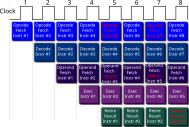
\includegraphics[width=0.6\textwidth]{pipeline-Struc-Hazard.pdf}
 \end{textblock*}
\end{frame}

\begin{frame}{Obstáculos Estructurales - Efecto en CPI}
 \begin{textblock*}{\textwidth}(0.3cm,1.2cm)
  \centering 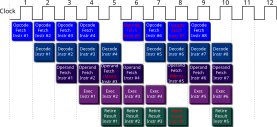
\includegraphics[width=0.7\textwidth]{pipeline-Struc-Hazard-effect1.pdf}\\
  \begin{itemize}[<+(1)->]\justifying
   \item Por cada Obstáculo, pospone una operación. $CPI = CPI+1$
   \item En general la cantidad de CPI que se incrementan es igual a la cantidad de concurrencias menos 1, en el lapso considerado
  \end{itemize}
 \end{textblock*}
\end{frame}

\begin{frame}{Obstáculos Estructurales - Efecto en CPI}
 \begin{textblock*}{\textwidth}(0.3cm,1.2cm)
  \centering 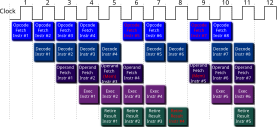
\includegraphics[width=0.7\textwidth]{pipeline-Struc-Hazard-effect2.pdf}\\
  \begin{itemize}\justifying
   \item Por cada Obstáculo, pospone una operación. $CPI = CPI+1$
   \item En general la cantidad de CPI que se incrementan es igual a la cantidad de concurrencias menos 1, en el lapso considerado
  \end{itemize}
 \end{textblock*}
\end{frame}

\begin{frame}{Obstáculos Estructurales - Efecto en CPI}
 \begin{textblock*}{\textwidth}(0.3cm,1.2cm)
  \centering 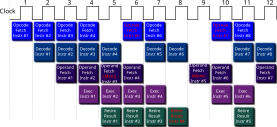
\includegraphics[width=0.7\textwidth]{pipeline-Struc-Hazard-effect3.pdf}
  \begin{itemize}
   \item Por cada Obstáculo, pospone una operación. $CPI = CPI+1$
   \item En general la cantidad de CPI que se incrementan es igual a la cantidad de concurrencias menos 1, en el lapso considerado
  \end{itemize}
 \end{textblock*}
\end{frame}

%%%%%%%%%%%%%%%%%%%%%%%%%%%%%%%%%%%% Nuevo Bloque 2 inicio
\begin{frame}{Obstáculos Estructurales - Posibles soluciones}
 \begin{textblock*}{\textwidth}(0.3cm,1.2cm)
   \begin{itemize}[<+(1)->]\justifying \parskip 0.2cm
   \item Cualquiera solución que implementemos,\textcolor{furfiBlue}{es necesario agregar hardware}.
   \item En el caso de accesos a memoria, se puede resolver mediante las siguientes opciones por separado o, \textcolor{furfiBlue}{por lo general}, combinadas:
   \begin{enumerate}
    \item Implementar el Modelo Harvard. Todos los procesadores modernos utilizan varios niveles de memorias Cache. El cache Level 1 lo desdoblan en Cache de datos y Cache de instrucciones.
    \item Empleo de \textcolor{furfiBlue}{buffers de instrucciones} implementados como pequeñas colas FIFO. Permiten no tener que fetchear a demanda sino en forma anticipada.
    \item Ensanchamiento de los buses mas allá de los anchos de palabra del procesador. Esta técnica de ``fuerza bruta'' \textcolor{furfiBlue}{complementa la solución de las FIFO de instrucciones ya que permite en un solo acceso fetchear varias instrucciones}.
   \end{enumerate}
   \item Aumentar \textcolor{furfiBlue}{equilibradamente} la profundidad del pipeline, \textcolor{furfiBlue}{produce etapas mucho mas simples capaces de resolver en un clock su tarea}.
  \end{itemize}
 \end{textblock*}
\end{frame}
 
\begin{frame}[fragile]{Obstáculos de datos}
 \begin{textblock*}{\textwidth}(0.3cm,1.2cm)
  \begin{itemize}[<+(1)->]\justifying
   \item Se producen cuando por \textcolor{furfiBlue}{efecto del pipeline}, una instrucción requiere de un dato antes de que este esté disponible por efecto de la secuencia lógica prevista en el programa.
   \item Consideremos el código que figura al pié. Corresponde a un procesador ARM.
   \item Se observa dependencias para el Registro R1. Hasta que la instrucción \textbf{\textit{add}} no complete su operación, R1 no tiene un valor válido. Por lo tanto \textcolor{furfiBlue}{no puede continuar} aplicándolo en las restantes que lo utilizan.
   \item La situación en el pipeline se muestra en el próximo slide.
  \end{itemize}
  \begin{onlyenv}<6->
   \lstset{language=[ARM]Assembler,numbers=none, escapechar=|}
   \begin{lstlisting}
add  R1,  R2, R3  ; R1 es el destino de esta operaci|\color{purple}\'o|n
sub  R4,  R1, R5  ; R1 es operando pero a|\color{purple}\'u|n no fue escrito el resultado
and  R6,  R1, R7  ;
orr  R8,  R1, R9  ; Se ejecutan finalizada la anterior
eor  R10, R1, R11 ;
   \end{lstlisting}
  \end{onlyenv}
 \end{textblock*}
\end{frame}
 
\begin{frame}{Obstáculos de Datos - Conflicto de recursos}
 \begin{textblock*}{\textwidth}(0.3cm,1.2cm)
  \centering 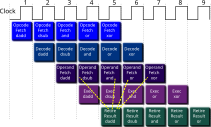
\includegraphics[width=0.67\textwidth]{pipeline-Data-Hazard.pdf}
 \end{textblock*}
\end{frame}
 
\begin{frame}{Obstáculos de Datos - Efecto en CPI}
 \begin{textblock*}{\textwidth}(0.3cm,1.2cm)
  \centering 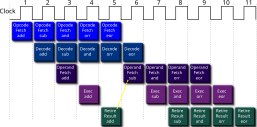
\includegraphics[width=0.77\textwidth]{pipeline-Data-Hazard-effect.pdf}
  \begin{itemize}\justifying
   \item Por cada Dependencia, pospone una operación. $CPI = CPI+n$, siendo $n$ la distancia entre las etapas del pipeline que requieren el mismo dato.
  \end{itemize}
 \end{textblock*}
\end{frame}
 
\begin{frame}{Solución a Obstáculos de Datos: Forwarding}
 \begin{textblock*}{.4\textwidth}(0.6cm,1.5cm)
  \centering 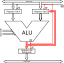
\includegraphics[width=\textwidth]{Forwarding.pdf}
 \end{textblock*}
 \begin{textblock*}{.57\textwidth}(6.7cm,1.2cm)
  \begin{itemize}[<+(1)->]\justifying \small
   \item Ni bien el resultado está disponible se lo realimenta a la entrada de la Unidad de Ejecución (ALU, FPU, etc.).
   \item Así, la etapa que lo requiere lo dispone en el mismo ciclo de clock en que se escribirá en el operando destino.
   \item Esto permite ahorrar el tiempo de escritura en el operando destino (No espera por el operando destino).
   \item Se aplica solamente a las etapas posteriores que quedarían en estado stall.
   \item Aquellas etapas que a pesar de la dependencia de datos, no quedarían en estado stall, reciben el resultado cuando este es aplicado en el operando destino.
  \end{itemize}
 \end{textblock*}
\end{frame}
 
\begin{frame}{Obstácualos de Datos - Forwarding}
 \begin{textblock*}{\textwidth}(0.3cm,1.2cm)
  \centering 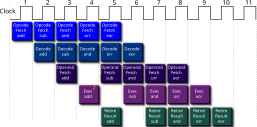
\includegraphics[width=.77\textwidth]{pipeline-Data-Hazard-forward.pdf}
  \begin{itemize}\justifying
    \item No resuelve completamente el problema pero reduce el efecto al 50\%.
   \end{itemize}
 \end{textblock*}
\end{frame}
 
\begin{frame}[fragile]{Algunas veces forwarding no es factible}
 \begin{textblock*}{\textwidth}(0.3cm,1.1cm)
  \begin{itemize}[<+(1)->] \justifying
   \item Normalmente forwarding aplica a operaciones de ALU denominadas back-to-back, ya que el bypass se efectúa desde la ALU a un registro entero del procesador.
   \item Consideremos ahora esta variante del código anterior.
\lstset{numbers=none,}
\vspace{-.3cm}
\begin{lstlisting}[escapechar=\|,label=noint]
ldr  R1,  [R2]    ;Lectura de memoria no pasa por la ALU.
sub  R4,  R1,  R5 ;R1 no puede ser forwardeado al ingresar.
and  R6,  R1,  R7
orr  R8,  R1,  R9
eor  R10, R1,  R11
\end{lstlisting}
\vspace{-.3cm}
   \item En este caso el dato proveniente de memoria es almacenado en el registro de datos que interfacea con el Bus de datos
   \item Desde este registro es enviado directamente al registro destino, en este caso R1.
   \item No puede adelantarse el valor a la siguiente etapa hasta que no se complete su escritura en R1.
  \end{itemize}
 \end{textblock*}
\end{frame}
 
\subsubsection{Mas problemas}
 
%%%%%%%%%%%%%%%%%%%%%%%%%%%%%%%%%%%%Nuevo Bloque 2 fin

\begin{frame}{Obstáculos de Control}
 \begin{textblock*}{\textwidth}(0.3cm,1.2cm)
  \begin{itemize}[<+->]\justifying \parskip 0.3cm
   \item La máquina de estados de un Pipeline busca instrucciones en forma secuencial.
   \item Un branch es una instrucción de control de flujo que provoca una discontinuidad en el flujo de ejecución.
   \item Un branch es la peor situación en pérdida de performance del Pipeline.
   \item El branch hace que todo lo que estaba pre procesado deba descartarse, ya que son las instrucciones sucesoras secuenciales al branch en el programa. Al interrumpirse la secuencia de ejecución, ya no son necesarias y deben ser reemplazadas por las instrucciones del target del branch.
   \item El pipeline se vacía. Se requieren \textbf{\textit{n -1}} ciclos de clock para obtener el próximo resultado, siendo \textit{\textbf{n}} la cantidad de etapas del pipeline. Esto se conoce como \textbf{\color{blue}branch penalty}.
  \end{itemize}
 \end{textblock*}
\end{frame}

\begin{frame}{"La conspiración de los branches"}
 \begin{figure}[ht!]
   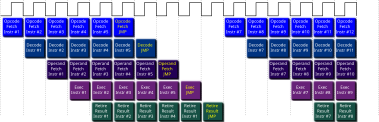
\includegraphics[width=0.95\textwidth]{pipeline-stalled.pdf}
 \end{figure}
\end{frame}


\begin{frame}{saltos, branches, interrupciones, llamadas...}
 \begin{textblock*}{\textwidth}(0.3cm,1.2cm)
  \begin{itemize} [<+(1)->] \justifying \parskip .1cm
   \item En las interrupciones la situación es la misma mostrada en el gráfico del slide anterior para los branches.
   \item En el caso de un branch el principal inconveniente se tiene cuando éste es condicional, ya que es necesario determinar si la condición es true o false.
   \item Si la condición es true se habla de \textbf{\textit{\color{blue}branch taken}}. Cambia el registro PC a la dirección de salto, y limpia el pipeline.
   \item Si resulta False se habla de \textbf{\textit{\color{blue}branch untaken}}. El PC que apunta a la instrucción siguiente al branch (la sucesora secuencial) se mantiene, y no se limpia el pipeline.
   \item Esta comprobación requiere llegar hasta la Etapa de ejecución del Pipeline.
   \item En el caso de un salto incondicional, o llamada a un procedimiento, en la etapa de decodificación ya se tiene la certeza que se producirá el salto, y solo se pierden menos elementos del Pipeline. Hay impacto de todos modos, pero de menor magnitud.
  \end{itemize}
 \end{textblock*}
\end{frame}
 
\begin{frame}{Efectos de los branches y como neutralizarlos}
 \begin{textblock*}{\textwidth}(0.3cm,1.2cm)
  \begin{itemize}[<+(1)->]\justifying \parskip 0.3cm
   \item Forwarding puede ayudar a disminuir el efecto de los diferentes casos expuestos anteriormente. Sin embargo, no es óptima, ya que solo lograremos disminuir algún ciclo de clock del \textbf{\color{blue}branch penalty}, pero siendo su efecto tan significativo, la modesta mejora que proporciona Forwarding termina siendo insuficiente.
   \item Para soluciones mas eficientes es necesario recurrir a análisis mas elaborados, que en general tienen en cuenta el comportamiento de los algoritmos y la frecuencia con que lso compiladores emplean instrucciones de salto.
   \item Ingresamos así al universo de las unidades de predicción de saltos. Las hay desde muy simples a muy sofisticadas, y tiene que ver no solo con las diferentes generaciones de procesadores, sino también con el tipo de procesador que se tome.
  \end{itemize}
 \end{textblock*}
\end{frame}

 %%%%%%%%%%%%%%%%%%%%%%%%%%%%%%%%%%%%%%%%%%%%%%%%%%%
\subsection{La memoria. El problema del acceso}

\begin{frame}{Ciclo de Bus de lectura}
 \begin{textblock*}{\textwidth}(0.4cm,1.2cm)
  \centering 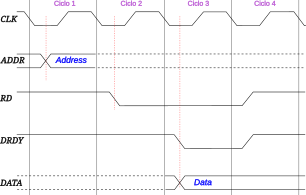
\includegraphics[width=.75\textwidth]{MemRDCycle.pdf}
 \end{textblock*}
\end{frame}

\begin{frame}{Ciclo de Bus de Escritura}
 \begin{textblock*}{\textwidth}(0.4cm,1.2cm)
  \centering 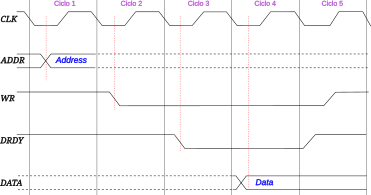
\includegraphics[width=.88\textwidth]{MemWRCycle.pdf}
 \end{textblock*}
\end{frame}

\begin{frame}{Performace Relativa Memoria DRAM vs. CPU}
 \begin{textblock*}{\textwidth}(0.4cm,1.2cm)
  \centering 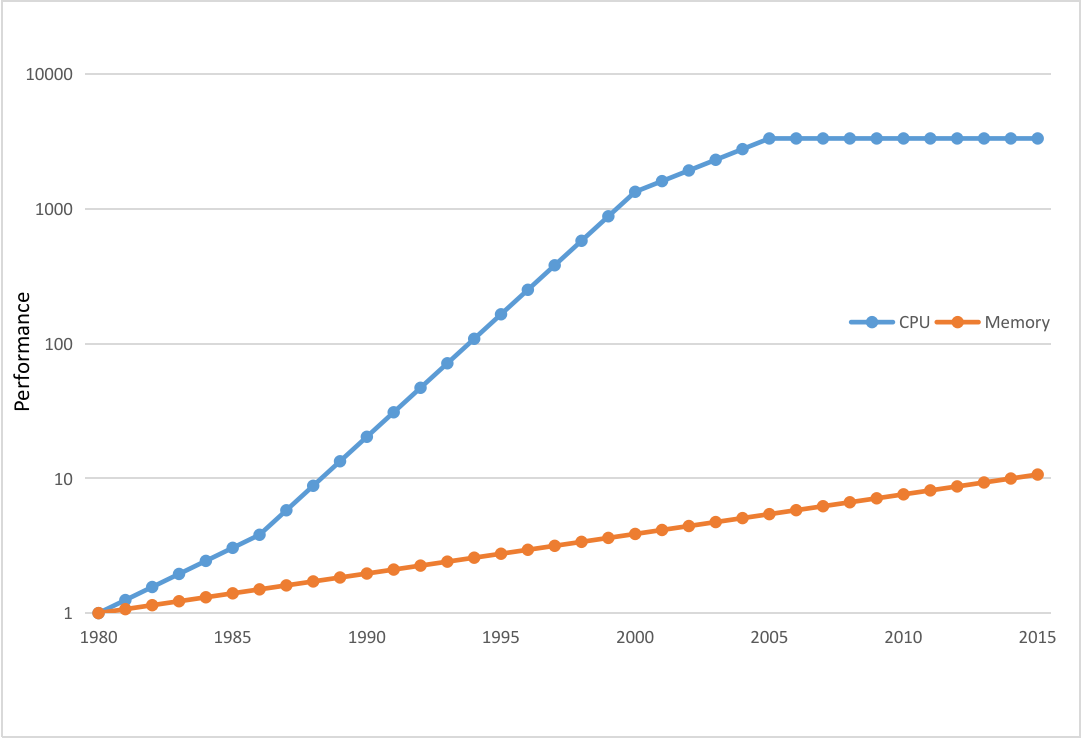
\includegraphics[width=.7\textwidth]{Mem-CPU-RelPerf.png}
 \end{textblock*}
\end{frame}

\begin{frame}{Performace Relativa Memoria DRAM vs. CPU. Notas}
 \begin{textblock*}{\textwidth}(0.4cm,1.2cm)
  \begin{itemize}[<+->]\justifying \parskip 0.15cm
   \item La escala logarítmica clarifica la magnitud del gap en performance.
   \item La progresión de memoria es a razón de 1.07 por año. Es constante, y parte de un baseline de \SI{64}{\kibi\byte} en 1980. Terminan en un incremento de aproximadamente x10.
   \item Para la CPU la base es de una sola CPU por sistema.
   \item El crecimiento tiene tramos diferentes: Hasta 1986 1,25 por año, luego hasta 2000 1.52 por año, entre 2000, y 2005 1.2, y a partir de ese año el mejoramiento de la performance entra en una meseta.
   \item Casualmente en ese año comienzan a presentarse los chips multicore.
  \end{itemize}
 \end{textblock*}
 \begin{textblock*}{\textwidth}(0.4cm,6.3cm)
  \only<6-> {
  \begin{block}{Conclusión}
   \justifying Necesitamos una estrategia de diseño para al menos minimizar el efecto de este gap.
  \end{block}
  }
  \only<7->{\vspace{-.3cm} \Large \centering \textit{\textbf{Continuará...}}}
 \end{textblock*}
\end{frame}
 %
% \begin{frame}{Algunas comparaciones de código}
%  Se requieren dos cosas:
%  \begin{enumerate}
%   \item Ingresar a \href{https://godbolt.org/}{Compiler Explorer}
%   \item Para sacar conclusiones útiles, pensar y aplicar lo que vimos hasta aqui.
%  \end{enumerate}
%
% \end{frame}
\section{Diseño de una CPU RISC}
\subsection{Diseño de un Pipeline simple}
\begin{frame}{CPU RISC = Pipeline simple}
 \begin{textblock*}{\textwidth}(0.3cm,1.2cm)
  \begin{itemize}[<+->] \justifying
   \item Utilizamos como base conceptual el procesador RISC-V, con arquitectura Load-Store, para ilustrar los conceptos básicos.
   \item Casi todas las ideas que presentamos son aplicables a otros procesadores, de arquitectura RISC, (como ARM y MIPS).
   \item La implementación es mucho más compleja con instrucciones más elaboradas.
   \item Las arquitecturas RISC se caracterizan por algunas propiedades clave:
   \begin{itemize}
    \item Todas las operaciones sobre datos se aplican a datos residentes en registros y, por lo general, modifican el registro completo (32 o \SI{64}{\bit}).
    \item Las únicas operaciones que afectan a la memoria son Load y Store, que mueven datos de la memoria a un registro o viceversa. Pueden involucrar menos de un registro completo (por ejemplo, \SI{1}{\byte}, \SI{16}{\bit} o \SI{32}{\bit}).
    \item Los formatos de instrucción son muy pocos, y todas las instrucciones suelen tener el mismo tamaño y layout. En RISC-V, los especificadores de registro: rs1, rs2 y rd, se ubican en la misma posición, lo que simplifica el control.
   \end{itemize}
   \item Estas propiedades simplifican drásticamente la implementación del pipeline.
  \end{itemize}
 \end{textblock*}
\end{frame}

\begin{frame}{Antes de pensar el Pipeline}
 \begin{textblock*}{\textwidth}(0.3cm,1.2cm)
  \begin{itemize}[<+->] \justifying
   \item Para comprender cómo se puede implementar un conjunto de instrucciones RISC en un pipeline, primero debemos entender cómo se implementa sin pipeline.
   \item Nuestra implementación no pipeline no es la más económica ni la de mayor rendimiento. Está diseñada para facilitar la transición a una implementación pipeline.
   \item La implementación del set de instrucciones requiere la introducción de varios registros temporales que no forman parte de la arquitectura.
   \item Se introducen para simplificar el \textcolor{Blue}{pipelining}.
   \item Nuestra implementación se centrará únicamente en un pipeline para un subconjunto de enteros de una arquitectura RISC que consta de operaciones Load-Store de palabras, saltos, y operaciones de la ALU de enteros.
   \item Implementación simple. Cada instrucción tarda como máximo 5 ciclos de reloj.
  \end{itemize}
 \end{textblock*}
\end{frame}

\begin{frame}{Pipeline. Etapa 1}
 \begin{textblock*}{.55\textwidth}(0cm,1.2cm)
  \begin{tcolorbox}[enhanced jigsaw,rounded corners, drop fuzzy shadow=ShadowColor]
   \textbf{\color{Blue}Ciclo de búsqueda de instrucciones (IF)}:

   Se envía el contador de programa (\textbf{\texttt{PC}}) a la memoria y se busca la instrucción actual.\\\

   El \textbf{\texttt{PC}} se actualiza a la siguiente instrucción secuencial sumándole 4 (ya que cada instrucción ocupa \SI{4}{\byte}).

  \end{tcolorbox}
 \end{textblock*}
 \begin{textblock*}{.5\textwidth}(0.55\textwidth,1.2cm)
  \centering 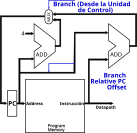
\includegraphics[width=\textwidth]{Datapath-PC.pdf}
 \end{textblock*}
\end{frame}

\begin{frame}{Pipeline. Etapa 2}
 \begin{textblock*}{\textwidth}(0.3cm,1.2cm)
  \begin{tcolorbox}[enhanced jigsaw,rounded corners, drop fuzzy shadow=ShadowColor]

   \textbf{\color{Blue}Ciclo de decodificación de instrucciones/búsqueda de registros (ID):}

   \begin{itemize}[<+(1)->]\justifying
    \item Se decodifica la instrucción y se leen del File Register los registros correspondientes a los especificadores Operando fuente u origen.
    \item Si la instrucción es un branch condicional, se realiza la prueba de igualdad en los registros a medida que se leen, para determinar si habrá branch. Si es necesario, se extiende el signo del campo de desplazamiento de la instrucción. Se calcula la dirección de destino del posible branch sumando el desplazamiento extendido al PC incrementado.
    \item La decodificación se realiza en paralelo con la lectura de registros, lo cual es posible porque los especificadores de registro se encuentran en una ubicación fija en una arquitectura RISC. Esta técnica se conoce como decodificación de campo fijo.
   \end{itemize}
  \end{tcolorbox}
 \end{textblock*}
\end{frame}

\begin{frame}{Pipeline. Etapa 2}
 \begin{textblock*}{\textwidth}(0.3cm,1.2cm)
  \begin{tcolorbox}[enhanced jigsaw,rounded corners, drop fuzzy shadow=ShadowColor]

   \textbf{\color{Blue}Ciclo de decodificación de instrucciones/búsqueda de registros (ID):}

   \begin{itemize}[<+(1)->]\justifying
    \item \textbf{\underline{Observación}}: Es posible que se lea un registro que luego no se utiliza. Esto no mejora el rendimiento, pero tampoco lo perjudica.

    (Leer un registro innecesario supone un desperdicio de energía, y los diseños que requieren un alto nivel de consumo energético deberían evitarlo).
    \item Para las operaciones de carga y las operaciones inmediatas de la ALU, el campo inmediato siempre se encuentra en la misma ubicación, por lo que podemos extender su signo fácilmente.

    Para una implementación más completa de RISC-V, necesitaríamos calcular dos valores con extensión de signo diferentes, ya que el campo inmediato para la operación de almacenamiento se encuentra en una ubicación distinta.
   \end{itemize}
  \end{tcolorbox}
 \end{textblock*}
\end{frame}

\begin{frame}{Pipeline. Etapa 3}
 \begin{textblock*}{\textwidth}(0.3cm,1.2cm)
  \begin{tcolorbox}[enhanced jigsaw,rounded corners, drop fuzzy shadow=ShadowColor]

   \textbf{\color{Blue}Ciclo de ejecución/dirección efectiva (EX):}

   \only<2->{La ALU opera sobre los operandos preparados en el ciclo anterior, realizando una de tres funciones, según el tipo de instrucción.}
   \begin{itemize}[<+(2)->]\justifying
    \item Referencia de memoria: La ALU suma el registro base y el desplazamiento para formar la dirección efectiva, que utilizará la etapa MEM.
    \item Instrucción ALU registro-registro: La ALU realiza la operación especificada por el código de operación, sobre los valores leídos del Register File.
    \item Instrucción ALU registro-inmediato: La ALU realiza la operación especificada por el código de operación, sobre el primer valor leído del Register File y el inmediato con extensión de signo.
    \item Salto condicional: Determina si la condición es verdadera.
   \end{itemize}
  \only<7->{En una arquitectura Load-Store, la dirección efectiva y los ciclos de ejecución se pueden combinar en un solo ciclo de reloj, ya que ninguna instrucción necesita calcular simultáneamente la dirección de datos y operar sobre ellos.}
  \end{tcolorbox}
 \end{textblock*}
\end{frame}

\begin{frame}{Pipeline. Etapa 4}
 \begin{textblock*}{\textwidth}(0.3cm,1.2cm)
  \begin{tcolorbox}[enhanced jigsaw,rounded corners, drop fuzzy shadow=ShadowColor]
   \textbf{\color{Blue}Acceso a memoria (MEM):}

   Si la instrucción es \textcolor{Blue}{Load}, la memoria realiza una lectura utilizando la dirección efectiva calculada en el ciclo anterior. Si es \textcolor{Blue}{Store}, la memoria escribe los datos del segundo registro leído del Register File utilizando la dirección efectiva.
  \end{tcolorbox}
 \end{textblock*}
\end{frame}

\begin{frame}{Pipeline. Etapa 5}
 \begin{textblock*}{\textwidth}(0.3cm,1.2cm)
  \begin{tcolorbox}[enhanced jigsaw,rounded corners, drop fuzzy shadow=ShadowColor]
   \textbf{\color{Blue}Ciclo de Write Back (WB):}

   \begin{itemize}[<+(1)->]\justifying
    \item Instrucción ALU de registro a registro o instrucción Load: Escribe el resultado en el File Register, ya sea que provenga del sistema de memoria (un Load) o de la ALU (una instrucción Aritmética o Lógica).
    \item En esta implementación, las instrucciones de salto requieren 3 ciclos, las de almacenamiento 4, y todas las demás instrucciones requieren 5 ciclos.
    \item Suponiendo una frecuencia de salto del 12 \% y una frecuencia de almacenamiento del 10 \%, una distribución típica de instrucciones resulta en un CPI general de 4,66.
    \item Sin embargo, esta implementación no es óptima ni por rendimiento ni por la mínima cantidad de hardware dado el nivel de rendimiento. Nos centramos en l aparalelización (pipelining) de esta versión.
   \end{itemize}
  \end{tcolorbox}
 \end{textblock*}
\end{frame}


\begin{frame}{Diseño de un DataPath Simple identificando el pipeline}
 \begin{textblock*}{\textwidth}(0.4cm,1.2cm)
  \centering 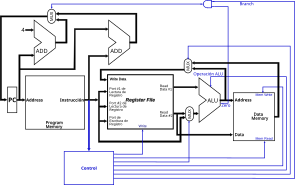
\includegraphics[width=.77\textwidth]{Datapath-2.pdf}
 \end{textblock*}
\end{frame}

\begin{frame}{Ejemplo de pipeline}
 \begin{textblock*}{\textwidth}(0.4cm,1.2cm)
  \centering 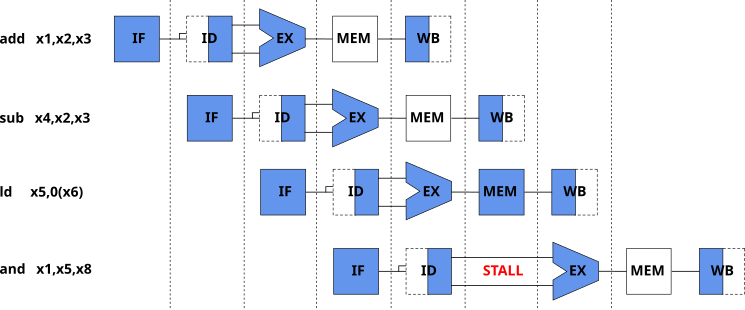
\includegraphics[width=.9\textwidth]{pipeline-Example1.pdf}
 \end{textblock*}
\end{frame}


\begin{frame}
 \Huge \centering ¿Preguntas?
\end{frame}


\end{document}
